%  LaTeX support: latex@mdpi.com
%=================================================================
\documentclass[appliedmath,article,submit,moreauthors]{Definitions/mdpi}

%=================================================================
% MDPI internal commands - do not modify
\firstpage{1}
\makeatletter
\setcounter{page}{\@firstpage}
\makeatother
\pubvolume{1}
\issuenum{1}
\articlenumber{0}
\pubyear{2026}
\copyrightyear{2026}
\datereceived{ }
\daterevised{ }
\dateaccepted{ }
\datepublished{ }

%=================================================================
% Additional packages not provided by the MDPI class
\usepackage{mathtools}
\usepackage{algorithm}
\usepackage{algpseudocode}
\usepackage{listings}
\usepackage{threeparttable}
\usepackage{csquotes}
\usepackage{amssymb}
\usepackage{tikz}
\usepackage{url}
\usetikzlibrary{shapes.geometric, arrows.meta, positioning}

\definecolor{LightGray}{RGB}{242,242,242}

\lstset{
  breaklines=true,
  breakatwhitespace=false,
  postbreak=\mbox{\textcolor{gray}{$\hookrightarrow$}\kern.5em},
  columns=fullflexible,
  keepspaces=true,
  backgroundcolor=\color{LightGray},
  frame=single,
  basicstyle=\ttfamily\footnotesize,
  language=Mathematica,
  keywordstyle=\color{blue},
  commentstyle=\color{gray!70},
  showstringspaces=false,
}

% Custom commands
\newcommand{\ord}{\mathrm{ord}}
\newcommand{\Z}{\mathbb{Z}}
\newcommand{\Q}{\mathbb{Q}}
\newcommand{\R}{\mathbb{R}}
\newcommand{\N}{\mathbb{N}}
\newcommand{\F}{\mathbb{F}}
\newcommand{\Ha}{\mathbb{H}}
\newcommand{\pil}{\pi_{\lambda,p}}
\newcommand{\pilb}{\bar{\pi}_{\lambda,p}}
\newcommand{\SL}{\operatorname{SL}}
\newcommand{\C}{\mathbb{C}}
\newcommand{\tor}{\mathrm{tor}}
\newcommand{\GL}{\operatorname{GL}}
\newcommand{\ZZ}{\mathbb{Z}}
\newcommand{\RR}{\mathbb{R}}
\newcommand{\NF}{\mathbb{N}}
\DeclareMathOperator{\Hom}{Hom}

\newcommand{\code}[1]{\colorbox{LightGray}{\nolinkurl{#1}}}
\newcommand*\rfrac[2]{{}^{#1}\!/_{#2}}

% Names of the verification layers
\newcommand{\Lean}{\textsc{Lean}}
\newcommand{\PALP}{\textsc{Palp}}
\newcommand{\Dq}{\Delta_q}
\newcommand{\relint}{\operatorname{relint}}
\newcommand{\interior}{\operatorname{int}}
\newcommand{\Conv}{\operatorname{conv}}

%================================================================
% Full title of the paper (Capitalized)
\Title{Classification of Five-Dimensional Reflexive Polytopes Arising from Single Weight Systems}

% Author ORCID IDs
\newcommand{\orcidauthorA}{0009-0003-8422-1272}
\newcommand{\orcidauthorB}{0000-0001-5257-2236}
\newcommand{\orcidauthorC}{0000-0001-6167-156X}

% Authors, for the paper
\Author{Andreas Hatziiliou $^{1}$\orcidA{}, Eldar Sultanow $^{2}$\orcidB{}, and Malik Amir $^{3,4,5}$\orcidC{}}

% Authors, for metadata in PDF
\AuthorNames{Andreas Hatziiliou, Eldar Sultanow, Malik Amir}

% Affiliations / Addresses
\address{%
$^{1}$ \quad Independent Researcher, Montreal QC, Canada\\
$^{2}$ \quad Chair of Business Informatics, Processes and Systems, University of
Potsdam, Karl-Marx-Stra{\ss}e 67, 14482 Potsdam, Germany\\
$^{3}$ \quad Faculty of Medicine, Université de Montréal, Montreal QC, Canada\\
$^{4}$ \quad Centre de Recherche du Centre Hospitalier de l'Université de
Montréal, Montreal QC, Canada\\
$^{5}$ \quad Centre Hospitalier Universitaire Sainte-Justine, Montreal QC, Canada}

% Contact information of the corresponding author
\corres{Correspondence: math@hatz.dev (A.H.); eldar.sultanow@wi.uni-potsdam.de (E.S.)}

% Abstract
\abstract{{\color{blue}We present a computational pipeline, along with two
layers of formal verification, for the exhaustive
\(\GL(5,\Z)\)-classification within the one-equation weight system sector in
dimension five: the Newton polytopes arising from the complete
Sch\"oller--Skarke list of length-six weight systems. The combined weight
systems and the subsequent reflexive-subpolytope search are not part of the
present computation, so the catalogues reported here are complete for the
single weight system sector and are explicitly \emph{not} a classification of
all five-dimensional reflexive polytopes.}
Starting from the Sch{\"o}ller--Skarke dataset of approximately $185$ billion reflexive
and $137$ billion IP weight systems, we compute the $\GL(5,\Z)$ normal form of
each associated
polytope, hash the resulting canonical matrix, and
deduplicate across the full dataset using a two-phase sort-merge
algorithm. The pipeline processes the $4.7$~TB input dataset across
distributed compute nodes, producing two single weight system catalogues:
$2{,}377{,}115{,}412$ unique reflexive polytopes and
$11{,}469{,}405{,}637$ unique IP polytopes (non-reflexive), each
with frequency counts and associated geometric invariants. Correctness
is established at two levels. At the theoretical level, we report a
\Lean~4 formalization of the Kreuzer--Skarke classification chain whose
main result is the \textcolor{blue}{\emph{completeness} of the
single weight system enumeration algorithm within this stated scope}.
At the level of the implementation, bounded model checking (CBMC) and
abstract interpretation (Frama-C) establish the correctness of the C/C++ models
and routines. }

% Keywords
\keyword{reflexive polytopes; lattice polytopes; Calabi--Yau manifolds; toric
geometry; weight systems; combined weight systems; classification; formal
verification; Lean; mirror symmetry; F-theory}

% MSC classification
\MSC{52B05; 52B55; 14J32; 14J33; 14M25; 68V20; 68Q60}

%%%%%%%%%%%%%%%%%%%%%%%%%%%%%%%%%%%%%%%%%%
\begin{document}

\section{Introduction}
\label{sec:intro}

Reflexive polytopes provide a fundamental bridge between discrete geometry and
the geometry of Calabi--Yau varieties. Their definition involves only lattices,
convexity, and polar duality, yet their consequences extend as far as toric
geometry, mirror symmetry, and string compactification theory. Let
\(M\simeq\Z^d\) be a lattice, let \(N=\operatorname{Hom}_{\Z}(M,\Z)\) be its
dual lattice, and write \(M_{\R}=M\otimes_{\Z}\R\) and
\(N_{\R}=N\otimes_{\Z}\R\). A full-dimensional lattice polytope \(\Delta\subset
M_{\R}\) containing the origin in its interior is called reflexive when its dual
polytope
\[
\Delta^*
=
\{y\in N_{\R}\mid \langle y,x\rangle\geq -1
\text{ for every }x\in\Delta\}
\]
is again a lattice polytope. Equivalently, every facet of \(\Delta\) lies at
lattice distance one from the origin.

The geometric significance of reflexivity is expressed by Batyrev's construction
of mirror Calabi--Yau hypersurfaces in toric varieties~\cite{Batyrev1994}. A
reflexive polytope \(\Delta\) determines a Gorenstein Fano toric variety whose
generic anticanonical hypersurface has trivial canonical class. Since the
ambient toric variety may be singular, one generally passes to a crepant toric
refinement, which preserves the canonical class and hence the Calabi--Yau
condition. The polar dual \(\Delta^*\) determines the mirror construction, with
the combinatorics of \(\Delta\) and \(\Delta^*\) exchanging complex-structure
and K\"ahler data. A classification of reflexive \(d\)-polytopes therefore
provides a classification of a large toric class of Calabi--Yau hypersurfaces of
dimension \(d-1\), together with their mirror duals.

Complete classifications are known only in dimensions at most four. There are
exactly \(16\) reflexive polygons in dimension two, explored independently by
Batyrev and Koelman~\cite{Batyrev1985,Koelman1991}. Kreuzer and Skarke
classified all \(4{,}319\) reflexive polytopes in dimension
three~\cite{KreuzerSkarke1998} and all \(473{,}800{,}776\) reflexive polytopes
in dimension four~\cite{KreuzerSkarke2000}. The four-dimensional Kreuzer--Skarke
database has become a standard source of toric Calabi--Yau threefold
hypersurfaces and has played a central role in the study of mirror symmetry,
toric fibrations, and string compactifications. The next case is dimension five,
where reflexive polytopes determine toric ambient fivefolds for Calabi--Yau
fourfold hypersurfaces, and the complete classification remains open.

The physical motivation for the five-dimensional case is that the Calabi--Yau
fourfolds arise naturally in M-theory compactifications to three dimensions and,
when equipped with suitable elliptic or genus-one fibrations and additional flux
data, in F-theory compactifications to four
dimensions~\cite{Vafa1996,MorrisonVafa1996I,MorrisonVafa1996II,BeckerBecker1996,BrunnerSchimmrigk1996,Weigand2018}.
The combinatorial catalogue does not by itself classify physical vacua, since
gauge sectors, charged matter, superpotentials, and other physical structures
depend on further geometric and flux choices, but it provides a large set of
candidate Calabi--Yau fourfold geometries. In this sense, it plays for fourfold
compactifications a role analogous to that of the four-dimensional
Kreuzer--Skarke database for Calabi--Yau threefolds.

Now, as opposed to the former case, we observe a severe combinatorial explosion
in dimension five. Sch\"oller and Skarke proposed the heuristic estimate
\(n_{\mathrm{RP}}(5)\gtrsim2^{2^6-4}=2^{60}\approx1.15\times10^{18}\) for the
number of five-dimensional reflexive polytopes~\cite{Scholler2019}. This scale
makes a direct enumeration unrealistic. Even under the optimistic assumption
that a canonical vertex matrix with approximately \(30\) vertices requires only
about \(150\) bytes, storing \(10^{18}\) polytopes would require on the order of
\(10^{20}\) bytes before metadata and indexing are included. Compared with a
global storage scale of order \(10^{23}\) bytes (a few zettabytes), such a
catalogue would occupy roughly 0.1\% of the total capacity. This calculation is
only illustrative, but it explains why the first feasible objective in dimension
five must be structural rather than exhaustive. A more data-informed estimate of
\(n_{\mathrm{RP}}(5)\) is discussed in \sect{sec:nrp5-estimate}.

The Kreuzer--Skarke \textcolor{blue}{classification} programme provides the required structural
framework. Instead of enumerating all reflexive polytopes directly, one first
determines the \(r\)-maximal reflexive polytopes from which all others can be
obtained as subpolytopes. A reflexive polytope is \(r\)-maximal when it is not
properly contained in a larger reflexive polytope on the same lattice. Polar
duality reverses inclusion, so \(r\)-maximal reflexive polytopes correspond to
\(r\)-minimal reflexive polytopes on the dual lattice. These \(r\)-minimal
objects are much easier to work with and were the main focus of the
classification efforts in $d=3,4$ as they contain vertex-minimal IP seeds, where
an IP polytope is a lattice polytope containing the origin in its interior and a
vertex-minimal IP polytope is one which loses this property whenever any vertex
is \textcolor{blue}{removed}. The clever construction of Kreuzer-Skarke leverages the fact that
these minimal IP seeds can all be encoded by weight systems and combined weight
systems, and their polar lattice hulls provide the polytopes on which the
\(r\)-maximal search is performed.

The four-dimensional classification illustrates the successive stages of this
method. They assembled \(201{,}346\) combined weight systems, of which
\(184{,}026\) were single weight systems and \(17{,}320\) were genuine
combinations. Among these, \(308\) CWS define the principal \(r\)-maximal Newton
polytopes on the finest compatible lattice, equivalently their polar duals are
principal \(r\)-minimal reflexive polytopes. Sublattice and quotient effects
contributed \(25\) further \(r\)-maximal polytopes, and the completed
classification produced another seven, giving \(340\) \(r\)-maximal reflexive
polytopes in total~\cite{KreuzerSkarke2000,KSFibrations2002,KreuzerCYData}.
Every four-dimensional reflexive polytope occurs as a reflexive subpolytope of
one of these maximal objects after the appropriate lattice realization is taken
into account.

In dimension five, the same strategy begins with a much larger and more delicate
collection of seed data. A vertex-minimal IP polytope in dimension \(d\) is
assembled from \(k\leq d\) IP simplices, possibly with shared vertices, and has
\(d+k\) vertices. The five-dimensional seeds therefore have between six and ten
vertices. The six-vertex case is simplicial and is encoded by length-six single
weight systems. Sch\"oller and Skarke enumerated \(322{,}383{,}760{,}930\) IP
weight systems of this type~\cite{Scholler2019}. Seeds with \(7,\ldots,10\)
vertices are encoded by combined weight systems assembled from lower-length IP
weight systems. The single weight system layer is therefore only the first part
of the five-dimensional classification, although its size already requires a
separate large-scale computation.

A further complication appears because the IP property no longer forces
reflexivity in dimension five. For the relevant Newton polytopes arising from
(combined) weight systems in dimensions at most four, every facet automatically
lies at lattice distance one from the origin~\cite{Skarke1996}. In dimension
five, an IP weight system may instead produce a Newton polytope with one or more
facets at greater lattice distance. Such a polytope is IP but not reflexive.
These non-reflexive polytopes cannot be discarded, since they may contain
reflexive subpolytopes that contribute to the eventual \(r\)-maximal list. 

The present paper classifies, up to \(\GL(5,\Z)\), the Newton polytopes arising
from length-six single weight systems in dimension five. It produces two
catalogues. The first contains the reflexive Newton polytopes arising from these
weight systems, while the second contains the IP but non-reflexive Newton
containers. The reflexive catalogue supplies the reflexive part of the
single weight system input to the \(r\)-maximal search, and the non-reflexive
catalogue records the additional containers that must be retained before
reflexive subpolytopes are enumerated.

{\color{blue}
\subsection{Terminology and scope.}
The foundational classification literature ordinarily uses \emph{weight
system} for one system of weights, while reserving \emph{combined weight
system} for a genuine combination of several such systems
~\cite{KS97,KreuzerSkarke1998,KreuzerSkarke2000,Scholler2019}. The phrase
\emph{single weight system} also occurs in that literature, but is used most
systematically in work where an explicit contrast is needed, notably
\cite{Avram1997}. We thus follow the standard  terminology
\emph{weight systems}; within the text we add \emph{single} whenever it helps
distinguish the one equation case from genuine CWS. Accordingly, every claim
of exhaustiveness in this article is relative to the full Sch\"oller--Skarke
list of \(322{,}383{,}760{,}930\) length-six weight systems. The paper does not
enumerate the CWS, quotients and sublattice
realizations arising from them, or the reflexive subpolytopes of the resulting
objects, and therefore does not claim a complete classification of all
five-dimensional reflexive polytopes.
}

Starting from the Sch\"oller--Skarke list of IP weight systems, the computation
is carried out by a distributed C++ pipeline that uses
{\color{blue}\PALP~\cite{PALP,GrinisKasprzyk2013} for lattice-polytope
operations and normal-form computation. \PALP\ is the de facto reference
implementation for the Kreuzer--Skarke framework: it was written by Kreuzer
and Skarke, evolved from the routines used in their reflexive-polytope
classification programme, and directly implements their vertex--facet pairing
matrix and lattice normal-form construction.} The pipeline uses \(128\)-bit
hashing for compact keys and external sort-merge deduplication for global
aggregation. For
each input weight system, the pipeline enumerates the lattice points of the
associated Newton polytope, computes its vertices and facets, tests the IP and
reflexivity conditions, constructs a canonical representative under
\(\GL(5,\Z)\), and records multiplicities together with lattice-point and vertex
data, dual data when the polar is a lattice polytope, and Batyrev--Hodge
invariants for the reflexive catalogue. The input contains
\(185{,}269{,}499{,}015\) weight systems producing reflexive Newton polytopes
and \(137{,}114{,}261{,}915\) producing IP but non-reflexive Newton containers;
after canonicalization and global deduplication, these yield
\(2{,}377{,}115{,}412\) distinct reflexive polytopes and
\(11{,}469{,}405{,}637\) distinct IP but non-reflexive polytopes.

Given the scale of this computation, correctness must be established from both
mathematical and implementation-level standpoints. The mathematical component
concerns the reduction from reflexive polytopes to minimal IP seeds and weight
systems. It is addressed through a \Lean~4 formalization of the relevant part of
the Kreuzer--Skarke reduction chain. The implementation component concerns
faithful execution without record loss, multiplicity corruption, or
nondeterministic canonicalization. It is addressed through bounded model
checking with CBMC~\cite{CBMC}, abstract interpretation and deductive
verification with Frama-C~\cite{FramaC}, global accounting identities, and
cross-validation against lower-dimensional data. These verification layers
provide independent evidence that the single weight system catalogues are
mathematically well specified and computationally reproducible.

The remainder of the paper is organized as follows. Section~\ref{sec:math}
develops the required lattice and toric geometry, including polar duality,
reflexivity, IP polytopes, (combined) weight systems and the distinction between
Newton polytopes and \(r\)-maximal reflexive polytopes.
Section~\ref{sec:pipeline} describes the computational pipeline, normal-form
construction, and global deduplication strategy. Section~\ref{sec:results}
presents the reflexive and IP but non-reflexive catalogues together with their
geometric and Hodge-theoretic statistics. Section~\ref{sec:verification}
explains the mathematical and implementation-level verification.
Sections~\ref{sec:discussion} and~\ref{sec:conclusion} discuss the implications
for the remaining CWS search and for the eventual \(r\)-maximal and complete
reflexive classifications.

\begin{figure}[H]
\centering
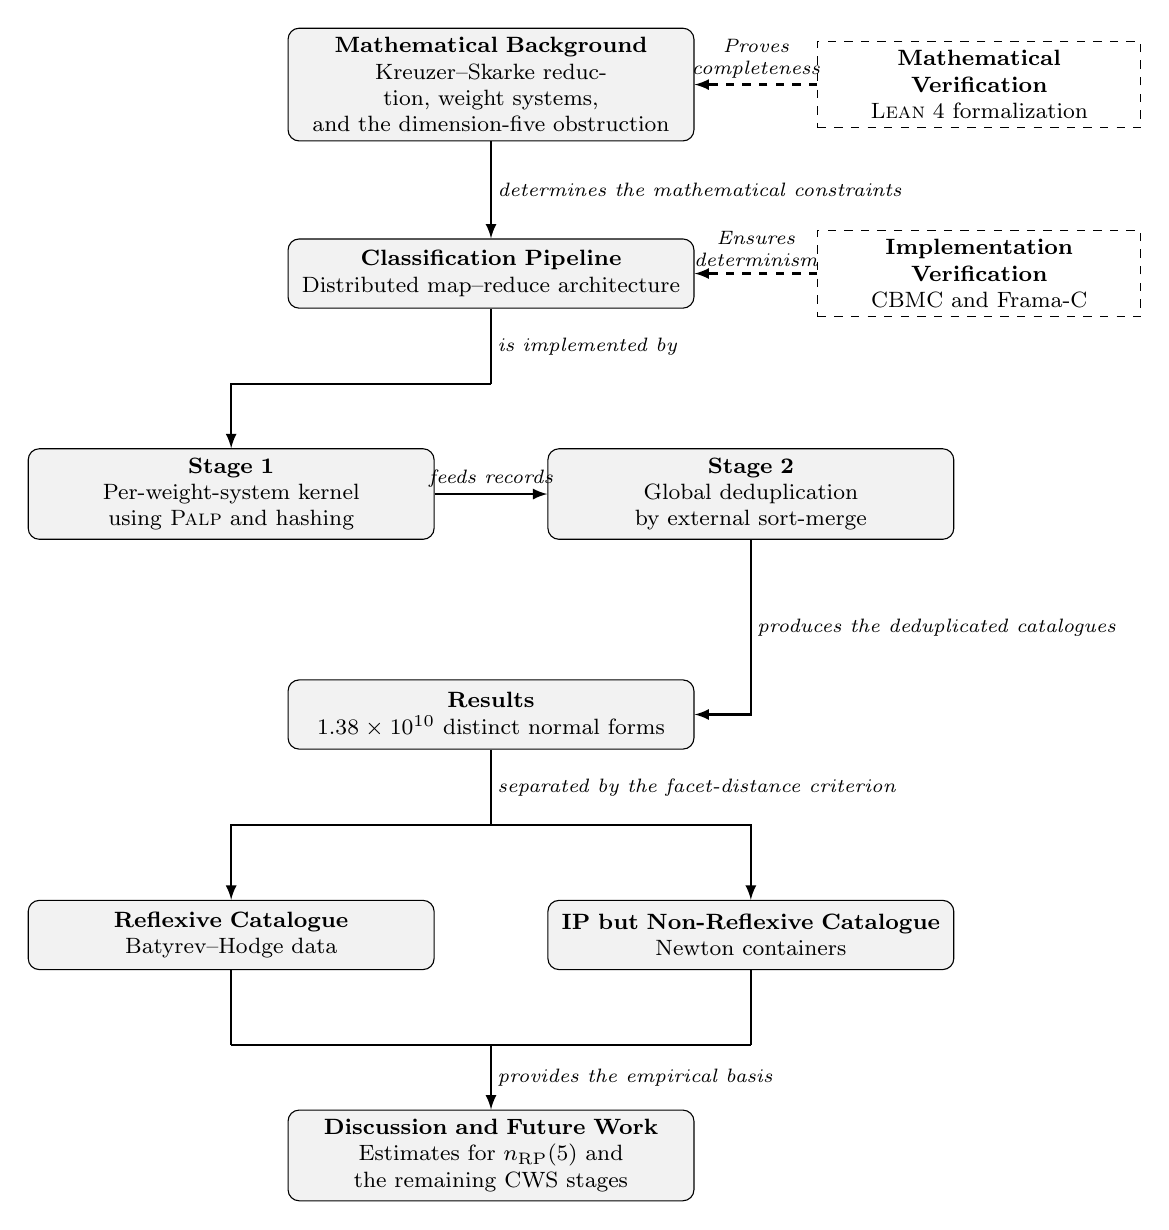
\begin{tikzpicture}[
    auto,
    block/.style={
        rectangle,
        draw,
        rounded corners,
        fill=LightGray,
        text width=14em,
        text centered,
        minimum height=2.5em,
        font=\footnotesize
    },
    verifblock/.style={
        rectangle,
        draw,
        dashed,
        fill=white,
        text width=11em,
        text centered,
        minimum height=2.5em,
        font=\footnotesize
    },
    line/.style={draw,-latex,thick},
    edgelabel/.style={
        font=\scriptsize\itshape,
        align=center,
        inner sep=2pt
    }
]

\node[block] (math) at (0,0)
{\textbf{Mathematical Background}\\
Kreuzer--Skarke reduction, weight systems,\\
and the dimension-five obstruction};

\node[block] (pipeline) at (0,-2.4)
{\textbf{Classification Pipeline}\\
Distributed map--reduce architecture};

\node[block] (stage1) at (-3.3,-5.2)
{\textbf{Stage 1}\\
Per-weight-system kernel using \PALP\ and hashing};

\node[block] (stage2) at (3.3,-5.2)
{\textbf{Stage 2}\\
Global deduplication by external sort-merge};

\node[block] (results) at (0,-8.0)
{\textbf{Results}\\
\(1.38\times10^{10}\) distinct normal forms};

\node[block] (cat_ref) at (-3.3,-10.8)
{\textbf{Reflexive Catalogue}\\
Batyrev--Hodge data};

\node[block] (cat_ip) at (3.3,-10.8)
{\textbf{IP but Non-Reflexive Catalogue}\\
Newton containers};

\node[block] (discussion) at (0,-13.6)
{\textbf{Discussion and Future Work}\\
Estimates for \(n_{\mathrm{RP}}(5)\) and the remaining CWS stages};

\node[verifblock] (verif_math) at (6.2,0)
{\textbf{Mathematical Verification}\\
\Lean~4 formalization};

\node[verifblock] (verif_impl) at (6.2,-2.4)
{\textbf{Implementation Verification}\\
CBMC and Frama-C};

\draw[line] (math) --
node[edgelabel,right]{determines the mathematical constraints}
(pipeline);

\draw[thick] (pipeline.south) --
node[edgelabel,right]{is implemented by}
(0,-3.8);

\draw[line] (0,-3.8) -| (stage1.north);

\draw[line] (stage1.east) --
node[edgelabel,above]{feeds records}
(stage2.west);

\draw[line] (stage2.south) |-
node[edgelabel,pos=0.25,right]{produces the deduplicated catalogues}
(results.east);

\draw[thick] (results.south) --
node[edgelabel,right]{separated by the facet-distance criterion}
(0,-9.4);

\draw[line] (0,-9.4) -| (cat_ref.north);
\draw[line] (0,-9.4) -| (cat_ip.north);

\draw[thick] (cat_ref.south) -- (-3.3,-12.2);
\draw[thick] (cat_ip.south) -- (3.3,-12.2);
\draw[thick] (-3.3,-12.2) -- (3.3,-12.2);

\draw[line] (0,-12.2) --
node[edgelabel,right]{provides the empirical basis}
(discussion.north);

\draw[line,dashed] (verif_math) --
node[edgelabel,above]{Proves \\ completeness}
(math);

\draw[line,dashed] (verif_impl) --
node[edgelabel,above]{Ensures \\ determinism}
(pipeline);

\end{tikzpicture}

\caption{Conceptual structure of the article. The mathematical foundations in
Section~\ref{sec:math} determine the classification pipeline in
Section~\ref{sec:pipeline}, which produces the reflexive and IP but
non-reflexive catalogues presented in Section~\ref{sec:results}. These
catalogues provide the empirical basis for the discussion and future work in
Sections~\ref{sec:discussion} and~\ref{sec:conclusion}. The mathematical and
implementation-level verification developed in Section~\ref{sec:verification}
addresses the theory and software independently.}
\label{fig:article_map_relations}
\end{figure}

\section{Mathematical Background}
\label{sec:math}

This section develops the mathematical framework underlying the computation. It
begins with lattice polytopes, polar duality, and reflexivity, which provide the
combinatorial foundation of Batyrev's construction of toric Calabi--Yau
hypersurfaces~\cite{Batyrev1994}. It then introduces the Kreuzer--Skarke
reduction from reflexive polytopes to maximal reflexive containers, minimal
objects on the polar side, vertex-minimal IP seeds, weight systems, and combined
weight systems~\cite{KS97,KreuzerSkarke2000,KSFibrations2002}. The later parts
of the section explain the additional obstruction appearing in dimension five,
the necessity of retaining IP but non-reflexive polytopes, and the use of
\(\GL(d,\Z)\)-normal forms for lattice-equivalence
testing~\cite{Skarke1996,Scholler2019,PALP}.

Throughout, \(M\simeq\Z^d\) denotes a lattice and
\(N=\operatorname{Hom}_{\Z}(M,\Z)\) its dual lattice. We write
\(M_{\RR}=M\otimes_{\Z}\RR\) and \(N_{\RR}=N\otimes_{\Z}\RR\), with the natural
pairing \(\langle\cdot,\cdot\rangle\colon N_{\RR}\times M_{\RR}\to\RR\). Thus
each \(y\in N_{\RR}\) is regarded as a real linear functional on \(M_{\RR}\),
and \(\langle y,x\rangle\) denotes its value on \(x\in M_{\RR}\).

\subsection{Lattice polytopes, polar duality, and reflexivity}
\label{sec:math-reflexive}

The interior point property is weaker than reflexivity, but it is the natural
starting point for the classification because vertex-minimal IP polytopes
provide the seeds from which the Kreuzer--Skarke construction produces maximal
Newton containers~\cite{KS97,KSFibrations2002}.

\begin{Definition}[Lattice polytope and IP property]
\label{def:lattice-polytope}
A \emph{lattice polytope} \(\Delta\subset M_{\RR}\) is the convex hull of
finitely many points of \(M\). It is full dimensional if its affine hull is
\(M_{\RR}\). The polytope has the \emph{interior point property}, or
\emph{IP property}, if \(0\in\interior(\Delta)\). If
\[
\Delta=\{x\in M_{\RR}\mid \langle a_F,x\rangle\geq-c_F
\text{ for every facet }F\},
\]
where each \(a_F\in N\) is the primitive inward normal to the facet \(F\), then
the IP property is equivalent to \(c_F>0\) for every facet.
\end{Definition}

Polar duality converts the facet inequalities of a polytope into vertices in the
dual vector space. It also reverses inclusions, thereby exchanging large objects
with small objects in the Kreuzer--Skarke reduction~\cite{Batyrev1994,KS97}.

\begin{Definition}[Polar dual]
\label{def:polar-dual}
Let \(\Delta\subset M_{\RR}\) be a full-dimensional polytope containing the
origin in its interior. Its \emph{polar dual} is
\[
\Delta^*=\{y\in N_{\RR}\mid \langle y,x\rangle\geq-1
\text{ for every }x\in\Delta\}.
\]
\end{Definition}

The distinction between the IP property and reflexivity is expressed by the
facet constants \(c_F\). The IP property requires only \(c_F>0\), whereas
reflexivity requires \(c_F=1\) for every facet. Geometrically, every facet of a
reflexive polytope lies at lattice distance one from the
origin~\cite{Batyrev1994,KS97}.

\begin{Definition}[Reflexive polytope]
\label{def:reflexive}
A full-dimensional lattice polytope \(\Delta\subset M_{\RR}\) with
\(0\in\interior(\Delta)\) is \emph{reflexive} if its polar dual
\(\Delta^*\subset N_{\RR}\) is also a lattice polytope. Equivalently, in the
primitive facet presentation of \(\Delta\), every facet constant satisfies
\(c_F=1\).
\end{Definition}

\begin{Proposition}[Involutivity, uniqueness, and inclusion reversal]
\label{prop:reflexive-properties}
Let \(\Delta\subset M_{\RR}\) be reflexive. Then the following statements hold.
\begin{enumerate}
    \item Polar duality is involutive, so \((\Delta^*)^*=\Delta\). In
    particular, reflexive polytopes occur in dual pairs \((\Delta,\Delta^*)\),
    with the roles of \(M\) and \(N\) exchanged.
    \item The origin is the unique interior lattice point of \(\Delta\).
    \item Polar duality reverses inclusion. If \(P\subseteq\Delta\) are
    full-dimensional polytopes containing the origin in their interiors, then
    \(\Delta^*\subseteq P^*\).
\end{enumerate}
\end{Proposition}

\begin{proof}
The identity \((\Delta^*)^*=\Delta\) is the bipolar theorem for closed convex
bodies containing the origin in their interiors. Since \(\Delta^*\) is a lattice
polytope by reflexivity and its polar is \(\Delta\), the dual polytope is itself
reflexive.

For uniqueness of the interior lattice point, let \(p\in M\) lie in
\(\interior(\Delta)\). For every vertex \(y\) of \(\Delta^*\), strictness of the
defining inequality gives \(\langle y,p\rangle>-1\). Since the pairing is
integral on \(N\times M\), one has \(\langle y,p\rangle\geq0\) for every vertex
\(y\) of \(\Delta^*\). If \(p\neq0\), the linear functional \(y\mapsto\langle
y,p\rangle\) would be nonnegative on the full-dimensional polytope \(\Delta^*\),
contradicting the fact that the origin lies in its interior. Hence \(p=0\).

Finally, if \(P\subseteq\Delta\), then every \(y\in\Delta^*\) satisfies
\(\langle y,x\rangle\geq-1\) for all \(x\in P\), and therefore \(y\in P^*\).
Thus \(\Delta^*\subseteq P^*\).
\end{proof}

The definitions above are formalized in \Lean\ as \nolinkurl{IsLatticePolytope},
\nolinkurl{IsIP}, \nolinkurl{polarDual}, and \nolinkurl{IsReflexive} in
\nolinkurl{Basic.lean}, and the three assertions of
Proposition \ref{prop:reflexive-properties} as the lemmas \nolinkurl{bipolar},
\nolinkurl{interior\_latticePoint\_unique}, and \nolinkurl{polarDual\_antitone},
as described in \sect{sec:verification-lean}.

\begin{Example}[The reflexive triangle of \(\mathbb{P}^2\)]
\label{ex:p2}
Let \(M=\Z^2\), and let \(\Delta\subset M_{\RR}\) be the triangle with vertices
\((-1,-1)\), \((2,-1)\), and \((-1,2)\). The origin is its unique interior
lattice point, and its polar dual has vertices \((1,0)\), \((0,1)\), and
\((-1,-1)\). Since the dual is also a lattice polygon, \(\Delta\) is reflexive.
This triangle is the two-dimensional toric model associated with
\(\mathbb{P}^2\) and illustrates the asymmetry that recurs in the
classification, where one member of the dual pair may be interpreted as an
anticanonical Newton polytope while the other carries the corresponding fan or
minimal seed data. This duality anticipates the maximal--minimal correspondence
developed in \sect{sec:math-chain}.
\end{Example}

\begin{figure}[H]
\centering

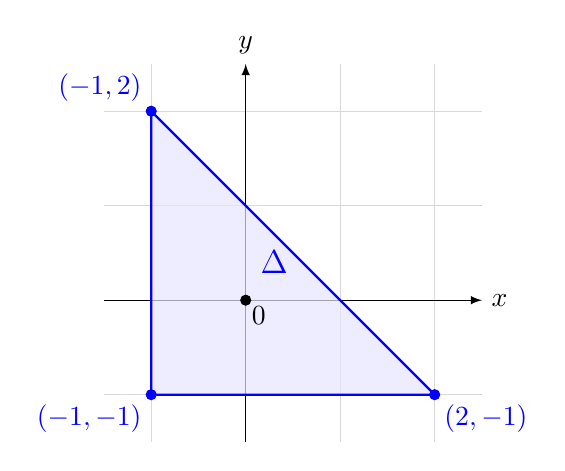
\begin{tikzpicture}[scale=1.2]
    \draw[step=1cm,gray!30,very thin] (-1.5,-1.5) grid (2.5,2.5);
    \draw[-latex] (-1.5,0) -- (2.5,0) node[right] {$x$};
    \draw[-latex] (0,-1.5) -- (0,2.5) node[above] {$y$};

    \draw[thick,blue,fill=blue!10,fill opacity=0.7]
        (-1,-1) -- (2,-1) -- (-1,2) -- cycle;

    \filldraw[black] (0,0) circle (1.5pt)
        node[anchor=north west,inner sep=2pt] {$0$};

    \filldraw[blue] (-1,-1) circle (1.5pt)
        node[below left] {$(-1,-1)$};
    \filldraw[blue] (2,-1) circle (1.5pt)
        node[below right] {$(2,-1)$};
    \filldraw[blue] (-1,2) circle (1.5pt)
        node[above left] {$(-1,2)$};

    \node[blue,font=\large] at (0.3,0.4) {$\Delta$};
\end{tikzpicture}
\hspace{1.5cm}
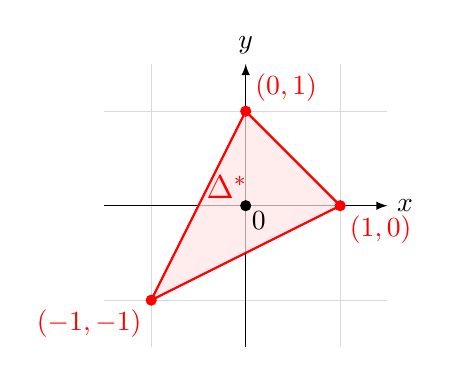
\begin{tikzpicture}[scale=1.2]
    \draw[step=1cm,gray!30,very thin] (-1.5,-1.5) grid (1.5,1.5);
    \draw[-latex] (-1.5,0) -- (1.5,0) node[right] {$x$};
    \draw[-latex] (0,-1.5) -- (0,1.5) node[above] {$y$};

    \draw[thick,red,fill=red!10,fill opacity=0.7]
        (1,0) -- (0,1) -- (-1,-1) -- cycle;

    \filldraw[black] (0,0) circle (1.5pt)
        node[anchor=north west,inner sep=2pt] {$0$};

    \filldraw[red] (1,0) circle (1.5pt)
        node[below right] {$(1,0)$};
    \filldraw[red] (0,1) circle (1.5pt)
        node[above right] {$(0,1)$};
    \filldraw[red] (-1,-1) circle (1.5pt)
        node[below left] {$(-1,-1)$};

    \node[red,font=\large] at (-0.2,0.2) {$\Delta^*$};
\end{tikzpicture}

\caption{The reflexive triangle \(\Delta\) associated with \(\mathbb{P}^2\) and
its polar dual \(\Delta^*\). The lattice grids show that the origin is the
unique interior lattice point of both polygons.}
\label{fig:p2_dual}
\end{figure}




\subsection{Calabi--Yau hypersurfaces and the Batyrev construction}
\label{sec:math-batyrev}

{\color{blue}Reflexive polytopes are fundamental in toric geometry because the
normal fan of a reflexive polytope defines a Gorenstein Fano toric variety, and
the polytope itself is the anticanonical polytope for that variety. The converse
requires this anticanonical normalization: the normal fan alone does not
determine the scale of a polytope. The anticanonical divisor is Cartier and
ample, and its generic members have trivial canonical class by
adjunction~\cite{Batyrev1994}.}

\begin{Theorem}[\textcolor{blue}{Reflexive anticanonical polytopes and
Gorenstein Fano toric varieties~\cite{Batyrev1994}}]
\label{thm:fano}
{\color{blue}
Let \(\Delta\subset M_{\RR}\) be a full-dimensional lattice polytope with
\(0\in\interior(\Delta)\), let \(\Sigma_{\Delta}\) be its normal fan, and let
\(\mathbb{P}_{\Delta}=X_{\Sigma_{\Delta}}\) be the associated toric variety.
Then \(\Delta\) is reflexive if and only if \(\mathbb{P}_{\Delta}\) is
Gorenstein Fano and, with the origin fixed as the unique interior lattice
point, \(\Delta\) is its anticanonical polytope
\[
P_{-K_{\mathbb{P}_{\Delta}}}
=
\{m\in M_{\RR}\mid \langle u_{\rho},m\rangle\geq-1
\text{ for every }\rho\in\Sigma_{\Delta}(1)\},
\]
where \(u_{\rho}\) is the primitive ray generator, using the inward-normal
convention. In this case the anticanonical divisor
\(-K_{\mathbb{P}_{\Delta}}\) is Cartier and ample, and the lattice points of
\(\Delta\cap M\) index a monomial basis of
\(H^0(\mathbb{P}_{\Delta},-K_{\mathbb{P}_{\Delta}})\). The anticanonical
normalization is essential: a nontrivial dilation of \(\Delta\) has the same
normal fan, but it is not the anticanonical polytope and need not be reflexive.
}
\end{Theorem}

\begin{Theorem}[Batyrev~\cite{Batyrev1994}]
\label{thm:batyrev}
Let \(\Delta\subset M_{\RR}\) be a reflexive polytope of dimension \(d\). A
generic member
\(X=\{\sum_{m\in\Delta\cap M}a_mx^m=0\}\subset\mathbb{P}_{\Delta}\) of the
anticanonical linear system has trivial canonical class. After passing to a
suitable projective crepant toric refinement, the proper transform defines a
Calabi--Yau hypersurface of dimension \(d-1\). It is a smooth Calabi--Yau
variety when a smooth crepant resolution exists, while in the general toric
setting its invariants are interpreted in the corresponding stringy sense.
\end{Theorem}

\begin{proof}
Since \(X\in|-K_{\mathbb{P}_{\Delta}}|\), the adjunction formula gives
\(K_X=(K_{\mathbb{P}_{\Delta}}+X)|_X=\mathcal{O}_X\). Thus the canonical bundle
of \(X\) is trivial. Reflexivity ensures that \(-K_{\mathbb{P}_{\Delta}}\) is
Cartier and ample, while a crepant toric refinement preserves the canonical
class. The proper transform therefore retains the Calabi--Yau condition.
\end{proof}

\begin{Example}[The quintic threefold]
\label{ex:quintic}
Let \(d=4\), and let \(\Delta\) be the reflexive simplex whose associated toric
variety is \(\mathbb{P}^4\). Since
\(-K_{\mathbb{P}^4}=\mathcal{O}_{\mathbb{P}^4}(5)\), a generic anticanonical
hypersurface is a quintic threefold in \(\mathbb{P}^4\). It is a Calabi--Yau
threefold with \(h^{1,1}=1\), \(h^{2,1}=101\), and Euler characteristic
\(\chi=2(h^{1,1}-h^{2,1})=-200\). This example is the classical model for
explicit calculations in mirror symmetry~\cite{Candelas1991}.
\end{Example}

\subsection{Hodge numbers and mirror symmetry}
\label{sec:math-hodge}

Batyrev's construction allows the Hodge numbers of a toric Calabi--Yau
hypersurface to be computed from the combinatorics of the dual pair
\((\Delta,\Delta^*)\)~\cite{Batyrev1994,BatyrevBorisov1996}. For a face
\(\Theta\), let \(\ell(\Theta)\) denote the number of lattice points of
\(\Theta\), let \(\ell^*(\Theta)\) denote the number of lattice points in its
relative interior, and let \(\Theta^*\) denote the face dual to \(\Theta\). If
\(X\) is the Calabi--Yau hypersurface associated with a \(d\)-dimensional
reflexive polytope, then for \(1\leq i\leq d-2\) Batyrev's formula is
\[
\begin{aligned}
h^{1,i}(X)={}&
\delta_{1i}
\left(
\ell(\Delta^*)-d-1-
\sum_{\operatorname{codim}\Theta^*=1}\ell^*(\Theta^*)
\right)
\\
&+
\delta_{d-2,i}
\left(
\ell(\Delta)-d-1-
\sum_{\operatorname{codim}\Theta=1}\ell^*(\Theta)
\right)
+
\sum_{\operatorname{codim}\Theta^*=i+1}
\ell^*(\Theta^*)\ell^*(\Theta).
\end{aligned}
\]
The symmetry of this expression under the exchange
\(\Delta\leftrightarrow\Delta^*\) is the combinatorial origin of mirror symmetry
in the toric hypersurface setting~\cite{Batyrev1994}. If \(X^*\) denotes the
hypersurface associated with \(\Delta^*\), then \(h^{1,1}(X)=h^{d-2,1}(X^*)\)
and \(h^{d-2,1}(X)=h^{1,1}(X^*)\).

For \(d=5\), the associated hypersurface is a Calabi--Yau fourfold whose
relevant Hodge numbers are \(h^{1,1}\), \(h^{1,2}\), \(h^{1,3}\), and
\(h^{2,2}\). In the smooth case they satisfy
\(h^{2,2}=44+4h^{1,1}-2h^{1,2}+4h^{1,3}\), while for singular toric
hypersurfaces the corresponding quantities are interpreted as stringy Hodge
numbers. Batyrev's construction supplied the first systematic large-scale source
of toric mirror pairs, and the Kreuzer--Skarke catalogues consequently became
central resources for the study of mirror
symmetry~\cite{KreuzerSkarke1998,KreuzerSkarke2000,KreuzerCYData}. The stronger
physical prediction involving the equality of quantum-corrected moduli spaces
was verified explicitly for the quintic by Candelas, de la Ossa, Green, and
Parkes~\cite{Candelas1991}.

\begin{Remark}[Calabi--Yau manifolds in physics]
A Calabi--Yau manifold is a compact K\"ahler manifold with trivial canonical
bundle. In the smooth simply connected case, this condition is equivalent to the
holonomy being contained in \(SU(n)\). Yau's theorem provides a Ricci-flat
K\"ahler metric in every K\"ahler class~\cite{Yau1978}. Compactification of
superstring theory on a Calabi--Yau threefold preserves \(\mathcal{N}=1\)
supersymmetry in four dimensions~\cite{Candelas1985}, with \(h^{1,1}\)
describing K\"ahler moduli and \(h^{2,1}\) describing complex-structure moduli.
Calabi--Yau fourfolds play the analogous geometric role in M-theory
compactifications and, when equipped with suitable elliptic or genus-one
fibrations and additional flux data, in F-theory
compactifications~\cite{Vafa1996,BeckerBecker1996,BrunnerSchimmrigk1996,Weigand2018}.
\end{Remark}



\subsection{The Kreuzer--Skarke reduction chain}
\label{sec:math-chain}

To classify reflexive polytopes, Kreuzer and Skarke introduced a novel reduction
chain that allows us to directly enumerate candidate (combined) weight systems
which give rise to $r$-minimal (resp. $r$-maximal) polytopes and which allow for
a complete classification~\cite{KS97,KreuzerSkarke2000,KSFibrations2002}.
Firstly, finiteness guarantees the existence of maximal reflexive polytopes,
which polar duality maps to minimal reflexive objects. These minimal objects
contain vertex-minimal IP seeds that decompose into IP simplices. Ultimately, IP
simplices are encoded by weight systems, and non-simplicial seeds are encoded by
combined weight systems.

\subsubsection{Finiteness}
\label{sec:math-finite}

\begin{Theorem}[Finiteness, Hensley and Lagarias--Ziegler]
\label{thm:finite}
For each fixed \(d\), the number of reflexive polytopes in \(\RR^d\), up to the
action of \(\GL(d,\Z)\), is finite.
\end{Theorem}

The proof proceeds in two steps. First, there exists a constant $c(d,k)$ such
that any $d$-dimensional lattice polytope with exactly $k\geq 1$ interior
lattice points has normalized volume at most $c(d,k)$. Because a reflexive
polytope has exactly one interior lattice point, its volume is bounded by a
constant depending only on $d$. Second, any lattice polytope of bounded
normalized volume is unimodularly equivalent to one contained in a fixed box
$[-R,R]^d$. Finiteness follows because there are only finitely many lattice
polytopes within such a bounded box~\cite{Hensley1983,LagariasZiegler1991}.

In \Lean, finiteness up to \(\GL(d,\Z)\) is proved as
\nolinkurl{finitely\_many\_reflexive} in \nolinkurl{Finiteness.lean}.  It is
derived from the two geometry-of-numbers inputs, the volume bound
\nolinkurl{hensley\_volume\_bound} and the box reduction
\nolinkurl{lagarias\_ziegler\_box}, which are imported as documented hypotheses,
together with the point-count bound \nolinkurl{latticePoint\_count\_bound}, as
described in \sect{sec:verification-lean}.

\begin{Remark}[Finiteness does not give an algorithm]
The constants in the general volume bounds are far too large to give a useful
enumeration by brute force.  The theorem is nevertheless essential because it
guarantees that ascending chains of reflexive polytopes terminate, that maximal
reflexive polytopes exist, and that deduplication modulo \(\GL(d,\Z)\) is a
finite classification problem~\cite{KS97,KreuzerSkarke2000}.  The termination of
ascending chains of lattice polytopes is formalized as
\nolinkurl{ncard\_lt\_of\_ssubset} in \nolinkurl{Finiteness.lean}.
\end{Remark}

\subsubsection{Subpolytope reduction}
\label{sec:math-subpolytope}

The classification first reduces to identifying reflexive polytopes that are
maximal under inclusion~\cite{KS97,KreuzerSkarke2000}.

\begin{Definition}[\(r\)-maximal reflexive polytope]
\label{def:rmaximal}
A reflexive polytope \(\Delta\subset M_{\RR}\) is called \emph{\(r\)-maximal} if
it is not properly contained in any larger reflexive polytope on the same
lattice.
\end{Definition}

\begin{Theorem}[Embedding into an \(r\)-maximal polytope]
\label{thm:embed}
Every reflexive polytope \(P\subset M_{\RR}\) is a subpolytope of some
\(r\)-maximal reflexive polytope \(\Delta\) on the same lattice.
\end{Theorem}

\begin{proof}
Enlarge \(P\) iteratively by proper inclusion into larger reflexive polytopes on
the same lattice. Because strict enlargement strictly increases normalized
volume, and the volume of reflexive polytopes in a fixed dimension is bounded,
this chain of inclusions must terminate. The terminal object is \(r\)-maximal.
\end{proof}

Thus the classification can be organized in two stages.  First one finds all
\(r\)-maximal reflexive polytopes.  Then one enumerates the reflexive
subpolytopes inside them~\cite{KreuzerSkarke2000}.  The embedding theorem is
formalized as \nolinkurl{exists\_maximal\_superset} in \nolinkurl{MaxMin.lean},
with the \(r\)-maximal condition defined as \nolinkurl{IsMaximalReflexive}.

\subsubsection{Max and min duality}
\label{sec:math-maxmin}

Polar duality reverses inclusion relations. Large maximal objects in \(M_{\RR}\)
correspond to small minimal objects in \(N_{\RR}\), and these smaller objects
are more constrained~\cite{KS97,KSFibrations2002}.

\begin{Definition}[\(r\)-minimal reflexive polytope]
\label{def:rminimal}
A reflexive polytope \(\nabla\subset N_{\RR}\) is called \emph{\(r\)-minimal} if
it contains no proper reflexive subpolytope.
\end{Definition}

\begin{Theorem}[Max and min duality]
\label{thm:maxmin}
Polar duality is an inclusion reversing bijection between reflexive polytopes in
\(M_{\RR}\) and reflexive polytopes in \(N_{\RR}\). A reflexive polytope
\(\Delta\subset M_{\RR}\) is \(r\)-maximal if and only if
\(\nabla=\Delta^*\subset N_{\RR}\) is \(r\)-minimal.
\end{Theorem}

\begin{proof}
If \(\Delta\subsetneq Q\) is a proper inclusion of reflexive polytopes in
\(M_{\RR}\), polar duality implies a proper inclusion \(Q^*\subsetneq\Delta^*\)
in \(N_{\RR}\). Conversely, any proper reflexive subpolytope of \(\Delta^*\)
dualizes to a proper reflexive enlargement of \(\Delta\). The absence of proper
reflexive enlargements of \(\Delta\) is therefore equivalent to the absence of
proper reflexive subpolytopes of \(\Delta^*\).
\end{proof}

This is the strategic inversion at the heart of the programme.  The
\(r\)-maximal Newton polytopes are often large and complicated, while their
polar duals are \(r\)-minimal and therefore much more constrained.  The next
step is to understand what these minimal dual objects contain.  Max and min
duality is formalized as \nolinkurl{maximal\_iff\_dual\_minimal} in
\nolinkurl{MaxMin.lean}, resting on the inclusion-reversal lemma
\nolinkurl{subset\_iff\_polarDual\_subset} and the self-duality of reflexivity
\nolinkurl{IsReflexive.polarDual\_reflexive}; the \(r\)-minimal condition is
defined as \nolinkurl{IsMinimalReflexive}.

\subsubsection{Vertex-minimal IP seeds}
\label{sec:math-vmin}

An \(r\)-minimal reflexive polytope need not itself be vertex-minimal as an IP
polytope.  Nevertheless, every IP polytope contains a vertex-minimal IP
subpolytope obtained by deleting vertices until no further deletion preserves
the IP property.  These smaller IP seeds are the objects that are directly
encoded by weight systems and combined weight systems~\cite{KS97}.  This descent
to a vertex-minimal seed is formalized as
\nolinkurl{exists\_minimalIPGen\_subset} in \nolinkurl{MaxMin.lean}, with the
vertex-minimal IP condition defined as \nolinkurl{IsMinimalIPGen} in
\nolinkurl{Minimal.lean}.

\begin{Definition}[Vertex-minimal IP polytope]
\label{def:vertex-minimal-ip}
Let \(\nabla=\Conv(V)\subset N_{\RR}\) be an IP polytope whose vertices are the
finite set \(V\).  We say that \(\nabla\) is \emph{vertex-minimal IP} if, for
every proper subset \(V'\subsetneq V\), the polytope \(\Conv(V')\) does not
contain the origin in its interior.
\end{Definition}

\begin{Theorem}[Structure of vertex-minimal IP polytopes~\cite{KS97}]
\label{thm:minstructure}
Let \(\nabla=\Conv(V)\subset N_{\RR}\) be a vertex-minimal IP polytope of
dimension \(d\).  Then \(V\) is a union of blocks $V=V_1\cup\cdots\cup V_k$
which are not required to be disjoint.  Each \(V_j\) is an affinely independent
set spanning a simplex $S_j=\Conv(V_j)$ whose relative interior contains the
origin.  Every vertex belongs to at least one block, and the partial spans
$\operatorname{span}(V_1\cup\cdots\cup V_j)$ increase strictly until they span
\(N_{\RR}\).  Moreover, $|V|=d+k,\, 1\leq k\leq d$ and hence $d+1\leq |V|\leq
2d$. If \(k=1\), then \(\nabla\) is a simplex.
\end{Theorem}

{\color{blue}
This theorem is a conventional mathematical result of Kreuzer and
Skarke~\cite{KS97}; the manuscript does not claim that every assertion in its
statement has already been proved in \Lean. The parts proved in the present
formalization are the lower bound \(d+1\leq|V|\), the simplicial case \(k=1\),
and the construction of normalized positive barycentric weights, through
\nolinkurl{minimalIPGen\_card\_lower},
\nolinkurl{simplex\_card}, and \nolinkurl{simplex\_weights} in
\nolinkurl{Minimal.lean}. The non-simplicial decomposition is represented by
the deferred theorem \nolinkurl{minimal\_structure}. Its iteration to the full
block decomposition, including the assertions \(|V|=d+k\) and
\(|V|\leq2d\), is therefore not yet machine-checked. These deferred
non-simplicial assertions are not used by the formally verified
single weight system (\(k=1\)) completeness theorem in this paper; they are
needed when the formalization is extended to the genuine CWS cases.
}

\begin{Example}[Simplex and product in dimension two]
\label{ex:minexamples}
In dimension two, the simplicial case has $V=\{(1,0),(0,1),(-1,-1)\}$. This is
the \(\mathbb{P}^2\) triangle and carries the single circuit relation
$(1,0)+(0,1)+(-1,-1)=0$. The product case has $V=\{(\pm 1,0),(0,\pm 1)\}$. It
carries two one dimensional circuit relations $(1,0)+(-1,0)=0$ and
$(0,1)+(0,-1)=0$, and the resulting square is the polytope associated with
\(\mathbb{P}^1\times\mathbb{P}^1\).
\end{Example}

Blocks sharing vertices first occur in dimension three with the classical
Egyptian pyramid configuration that consists of two triangles \(V_1V_2V_3\) and
\(V_1V_2'V_3'\) with a common apex \(V_1\). It is a vertex-minimal IP polytope
with \(5=d+2\) vertices whose two simplex blocks overlap.  This is why Theorem
\ref{thm:minstructure} must allow non-disjoint blocks~\cite{KS97}.

\subsection{Weight systems}
\label{sec:math-weights}

A weight system is the arithmetic record of an IP simplex.  If the origin lies
in the relative interior of a simplex, then its barycentric coordinates with
respect to the vertices are positive.  Clearing denominators turns these
barycentric coordinates into integral weights~\cite{Skarke1996,Conrads2002}.

\begin{Definition}[Weight system]
\label{def:weights}
A \emph{weight system} of length \(d+1\) is a tuple \(q=(q_0,\ldots,q_d)\) of
positive rational numbers satisfying \(\sum_i q_i=1\). Equivalently, it may be
written as a tuple of coprime positive integers \((w_0,\ldots,w_d)\) with
\(q_i=w_i/D\) and \(D=\sum_i w_i\). If \(v_0,\ldots,v_d\) are affinely
independent vertices, the weight system records the circuit relation \(\sum_i
w_i v_i=0\). It also defines the weighted projective space
\(\mathbb{P}^d_{(w_0,\ldots,w_d)}\).
\end{Definition}

\begin{Lemma}[Interior point criterion]
\label{lem:ipcrit}
{\color{blue}Let \(v_0,\ldots,v_d\in\RR^d\) be the vertices of a non-degenerate
simplex, so that they are affinely \emph{independent} and their affine hull is
all of \(\RR^d\). Regarded as \(d+1\) vectors in \(\RR^d\) they are necessarily
\emph{linearly} dependent, so a nontrivial relation \(\sum_i w_iv_i=0\) exists.
Affine independence implies both that the space of such relations is
one-dimensional and that \(\sum_iw_i\neq0\) for every nontrivial relation;
after rescaling we may therefore write \(\sum_iw_i=c>0\), and \(w\) is then
unique up to a positive scalar.} Then
\(0\in\interior\Conv\{v_0,\ldots,v_d\}\) if and only if \(w_i>0\) for every
\(i\).
\end{Lemma}


\begin{proof}
{\color{blue}We first verify the two assertions about the relation. Let \(A\) be
the \(d\times(d+1)\) matrix with columns \(v_0,\ldots,v_d\). Affine
independence means that \(v_1-v_0,\ldots,v_d-v_0\) are linearly independent, so
the column space of \(A\) is all of \(\RR^d\) and \(\operatorname{rank}A=d\); hence
\(\dim\ker A=(d+1)-d=1\), which is the asserted uniqueness up to scaling. If
some nontrivial \(w\in\ker A\) had \(\sum_iw_i=0\), then \(\sum_iw_iv_i=0\)
would be a nontrivial \emph{affine} dependence among \(v_0,\ldots,v_d\),
contradicting affine independence; hence \(\sum_iw_i\neq0\), and replacing
\(w\) by \(-w\) if necessary gives \(c=\sum_iw_i>0\).}

For a simplex, barycentric coordinates are unique, and a point lies in the
interior if and only if all of its barycentric coordinates are positive.
Normalizing the linear relation by \(c=\sum_i w_i\) and setting
\(\lambda_i=w_i/c\) gives \(\sum_i \lambda_i v_i=0\) and \(\sum_i \lambda_i=1\).
Thus the \(\lambda_i\) are the barycentric coordinates of the origin. Therefore
the origin lies in the interior if and only if \(\lambda_i>0\) for every \(i\),
which is equivalent to \(w_i>0\) for every \(i\).
\end{proof}

{\color{blue}
More explicitly, let \(\lambda_0,\ldots,\lambda_d\) be the unique barycentric
coordinates of the origin with respect to the simplex. Because the vertices are
lattice points, these coordinates are rational. Choose a common denominator
\(L>0\), set \(a_i=L\lambda_i\), and divide the positive integer tuple
\((a_0,\ldots,a_d)\) by \(g=\gcd(a_0,\ldots,a_d)\). This gives the primitive
positive integer relation
\[
    \sum_{i=0}^{d}w_i v_i=0,
    \qquad
    \gcd(w_0,\ldots,w_d)=1.
\]
Writing \(D=\sum_i w_i\), the normalized rational weight system is
\(q_i=w_i/D=\lambda_i\), so \(\sum_iq_i=1\). Since the space of linear
relations among the \(d+1\) simplex vertices is one-dimensional, every positive
integral relation is a positive multiple of this one. The primitive integer
weights, and hence the normalized rational weights, are therefore unique up to
the ordering of the vertices.
}

Thus the IP property of a simplex is encoded by the signs of the coefficients in
its unique {\color{blue}linear relation}.  This criterion is the geometric engine of the
weight system enumeration~\cite{Skarke1996,Scholler2019}, and it is formalized
as \nolinkurl{ip\_simplex\_iff\_weights\_pos} in \Lean, as described in
\sect{sec:verification-lean}.  The identification of the weights with the
barycentric coordinates of the origin is \nolinkurl{simplex\_weights} in
\nolinkurl{Minimal.lean}.

\subsection{The pruning bound \texorpdfstring{\(q_i\leq 1/2\)}{qi <= 1/2}}
\label{sec:math-half-bound}

The enumeration of weight systems relies on elementary pruning bounds. The most
basic one says that no weight in an IP weight system can exceed one
half~\cite{Skarke1996,Scholler2019}.

\begin{Proposition}[Necessary half weight bound]
\label{prop:halfbound}
If \(q\) is an IP weight system, then \(q_i\leq 1/2\) for every \(i\). If some
\(q_i>1/2\), then every monomial solution of \(q\cdot x=1\) has
\(x_i\in\{0,1\}\), so the point \((1,\ldots,1)\) lies on the boundary in the
\(x_i\) direction and the origin cannot be interior after the standard shift.
\end{Proposition}

\begin{proof}
If \(q_i>1/2\) and \(x_i\geq 2\), then \(q\cdot x>1\), because all weights and
coordinates are nonnegative. Hence every nonnegative integer solution of
\(q\cdot x=1\) has \(x_i=0\) or \(x_i=1\). Therefore the degree slice has no
lattice points on one side of the affine hyperplane \(x_i=1\). After shifting by
\((1,\ldots,1)\), the candidate interior point becomes the origin and lies on a
supporting hyperplane rather than in the interior. This contradicts the IP
property.
\end{proof}

In integral notation, this gives the bound \(w_i\leq D/2\).  In the sorted
recursive enumeration one also uses the sharper slot bound
\[
        w_i\leq \frac{D}{d+1-i}.
\]
The boundary case \(q_i=1/2\) is special.  It is handled by reducing to a search
of one lower length with total weight \(1/2\), after which the half weight is
appended~\cite{Skarke1996,Scholler2019}.  The half weight obstruction is
formalized in \Lean\ as \nolinkurl{not\_ip\_of\_weight\_gt\_half}, the fact that
at most one weight can equal \(1/2\) as \nolinkurl{at\_most\_one\_half}, and the
reduction itself as the deferred statement \nolinkurl{ip\_half\_reduction}, all
in \nolinkurl{WeightSystem.lean}.

\subsection{The two polytope subtlety}
\label{sec:math-two-polytope}

A single weight system determines two related but distinct polytopes, and the
distinction between them is essential for separating the minimal side of the
Kreuzer--Skarke reduction from the Newton polytope computed by the
classification pipeline~\cite{KS97,KSFibrations2002,Scholler2019}. The first
object is the minimal IP simplex encoded by the positive circuit relation
$\sum_i w_i v_i=0$, whose vertices $v_i$ span a simplex containing the origin in
its relative interior. In dimension five, a single weight system has length six,
so this simplex has six vertices.

The second object is the associated maximal Newton polytope. Writing
$W_q=\{y\in\RR^n\mid \sum_i q_i y_i=0\}$, one defines
$\Dq=\Conv\bigl(\Z^n\cap\{y\in W_q\mid y_i\geq -1\text{ for every }i\}\bigr)$.
After the shift $x=y+\mathbf{1}$, the lattice points of $\Dq$ correspond to the
nonnegative integer solutions of $\sum_i q_i x_i=\sum_i q_i$. If $q_i=w_i/D$,
these solutions are precisely the monomials of weighted degree $D$ in the
corresponding weighted polynomial ring~\cite{Skarke1996,Conrads2002}.

The minimal IP simplex and the Newton polytope $\Dq$ therefore encode different
parts of the construction. The simplex records the positive {\color{blue}linear relation}
among the minimal generating vertices, whereas $\Dq$ is the lattice hull of all
degree-$D$ monomials in the weight hyperplane. In the dual construction, the
simplex determines the rational polar body whose lattice hull is $\Dq$, and the
classification pipeline reconstructs and tests $\Dq$ rather than the simplex
alone. Accordingly, the statement that a single weight system corresponds to a
simplex refers to the minimal IP seed, while statements about the number of
vertices or lattice points refer to the maximal Newton polytope $\Dq$. Its polar
dual $\Dq^*$ is a further polytope in the dual lattice, with facets
corresponding to the vertices of $\Dq$.


\subsection{Combined weight systems}
\label{sec:math-cws}

When a vertex-minimal IP polytope is not a simplex, it cannot be described by a
single weight vector. The Kreuzer--Skarke structure theorem shows that such a
polytope is assembled from several IP simplices, possibly with shared vertices,
and a combined weight system records both the weight system attached to each
simplex block and the pattern of overlap among the
blocks~\cite{KS97,KSFibrations2002}.

\begin{Definition}[Combined weight system]
\label{def:cws}
A \emph{combined weight system}, or \emph{CWS}, in dimension \(d\) is a
collection of weight systems \(q^{(1)},\ldots,q^{(k)}\) supported on subsets
\(B_1,\ldots,B_k\) of a common coordinate set of size \(n=d+k\), with the
supports covering the full coordinate set. Each block is individually IP, and
overlaps among the supports encode vertices shared by the corresponding
simplices. Writing the combined weights as a \(k\times n\) matrix \(W\), with
\(q_i^{(a)}=0\) for \(i\notin B_a\), the associated CWS polytope lies in the
joint kernel \(\bigcap_{a=1}^k\{y\mid \langle W_a,y\rangle=0\}\), which has
dimension \(n-k=d\), and it has the IP property precisely when the origin lies
in its interior.
\end{Definition}

{\color{blue}
A vertex-minimal IP polytope with \(k\) simplex blocks has \(d+k\) vertices.
The case \(k=1\) gives the \((d+1)\)-vertex simplex encoded by one weight
system. The cases \(k=2,\ldots,d\) give non-simplicial seeds with
\(d+2,\ldots,2d\) vertices and are encoded by genuine combined weight systems:
each simplex block contributes one row of the CWS matrix, and overlaps of their
supports record vertices shared by different blocks. Thus, in dimension five,
\(k=1\) gives the six-vertex single weight system sector classified in this
paper, whereas \(k=2,\ldots,5\) give the seven- through ten-vertex CWS sectors.
Those sectors are described to locate the present result within the complete
Kreuzer--Skarke programme, but they are not computational outputs of this
paper; their enumeration and classification remain subsequent
work~\cite{KS97,Scholler2019}.
}

The four-dimensional classification illustrates the role of these objects
concretely. The complete CWS census consists of \(184{,}026\) single weight
systems and \(17{,}320\) genuine combined weight systems. Among the genuine CWS,
\(16{,}040\) are of type \(4+4\), \(1{,}122\) are of type \(4+3\), \textcolor{blue}{six are} of
type \(3+3\), \(36\) are of type \(3+3+3\), and \(116\) arise by adjoining a
segment block of type \((1,1)\) to three-dimensional structures. Altogether,
this yields \(201{,}346\) IP combined weight systems in dimension four
~\cite{KreuzerSkarke2000,KSFibrations2002,KreuzerCYData}.

Since every block in a CWS with \(k\geq2\) is a simplex of dimension at most
\(d-1\), the blocks occurring in dimension five are drawn from the already known
IP weight systems of lengths \(2,\ldots,5\), while only the length-six single
weight systems required the large-scale Sch\"oller--Skarke
enumeration~\cite{Scholler2019}. Every block of an IP combined weight system is
itself an IP weight system, a fact formalized in \Lean\ as
\nolinkurl{cws\_ip\_component}. The converse statement that every minimal IP
polytope admits such a decomposition into simplex blocks is the Kreuzer--Skarke
structure theorem, corresponding to Lemma~1 and its corollaries in~\cite{KS97},
and remains the principal open theorem in the present formalization under the
name \nolinkurl{minimal\_structure}, as discussed in
\sect{sec:verification-lean}.

\subsection{\texorpdfstring{\(r\)-maximal}{r-maximal} coverage by minimal IP containers}
\label{sec:math-containers}

The preceding constructions describe the minimal seed data, and the next step is
to explain how these seeds produce containers that cover all \(r\)-maximal
reflexive polytopes. If \(S\subset N\) is a finite set such that \(\Conv(S)\)
has the IP property, then \(\Conv(S)^*\subset M_{\RR}\) is a rational polytope,
and the associated lattice Newton container is defined by \(C(S)=[\Conv(S)^*]\),
where \([\cdot]\) denotes the convex hull of the lattice points of the enclosed
polytope~\cite{KS97,KSFibrations2002}.

\begin{Theorem}[\(r\)-maximal coverage by minimal IP containers]
\label{thm:rmaximal-pipeline}
Let \(P\subset M_{\RR}\) be an \(r\)-maximal reflexive polytope. Then there
exists a minimal IP generating set \(S\subset P^*\) such that \(P\subseteq
C(S)=[\Conv(S)^*]\). Moreover, if \(Q\) is reflexive and satisfies \(P\subseteq
Q\subseteq C(S)\), then \(Q=P\).
\end{Theorem}

\begin{proof}
Since \(P^*\) is reflexive, it has the IP property, and its lattice points
therefore contain a minimal IP subset \(S\). The inclusion \(\Conv(S)\subseteq
P^*\) and the inclusion-reversing property of polar duality imply
\(P=P^{**}\subseteq\Conv(S)^*\). Because \(P\) is a lattice polytope, passing to
the convex hull of lattice points preserves this inclusion, so
\(P\subseteq[\Conv(S)^*]=C(S)\). If \(Q\) is reflexive and \(P\subseteq Q\),
then the \(r\)-maximality of \(P\) forces \(Q=P\). The additional condition
\(Q\subseteq C(S)\) specifies the container in which the search is performed but
is not needed for the final maximality argument.
\end{proof}

The theorem does not require the container \(C(S)\) to be reflexive, and this
point is essential in dimension five. An IP but non-reflexive Newton container
may contain reflexive subpolytopes, and some of these may contribute to the
eventual \(r\)-maximal list~\cite{Skarke1996,Scholler2019}. The finite range of
possible seeds is controlled by the bound \(|S|\leq 2d\). Hence, in dimension
five, the complete minimal-IP seed data consists of the six-vertex
single weight system case and the CWS cases with \(7,\ldots,10\) vertices,
together with the quotient and sublattice realizations encoded by the CWS
lattice data~\cite{KS97,KSFibrations2002}.

The \Lean\ formalization proves the coverage and maximality statement as
\nolinkurl{maximal\_reflexive\_covered\_by\_minimalIP\_container}, a consequence
of the general coverage theorem \nolinkurl{classification\_coverage} in
\nolinkurl{Classification.lean}; the pseudoreflexivity identity underlying the
lattice-hull container operation \([\cdot]\) is \nolinkurl{pseudoreflexive} in
\nolinkurl{WeightSystem.lean}. The \(2d\) CWS vertex bound depends on the still
deferred theorem \nolinkurl{minimal\_structure}.

\begin{Remark}[\(r\)-minimal and vertex-minimal are different notions]
\label{rmk:rmin-vs-vmin}
The bound \(2d\) applies only to vertex-minimal IP seeds. An \(r\)-minimal
reflexive polytope contains no proper reflexive subpolytope, but it may contain
a vertex-minimal IP seed as a proper subpolytope and may also contain proper IP
subpolytopes that are not reflexive. Therefore an \(r\)-minimal reflexive
polytope need not be vertex-minimal as an IP polytope, and its number of
vertices is not bounded by \(2d\).

Running \PALP\ over the \(308\) published four-dimensional CWS whose Newton
polytopes define the principal \(r\)-maximal containers shows that the
corresponding dual \(r\)-minimal polytopes \((\Dq)^*\) have between five and
nine vertices. Eleven of them have \(9>2d=8\) vertices, so \(r\)-minimal
polytopes in dimension five may likewise have more than ten
vertices~\cite{KreuzerSkarke2000,KSFibrations2002,PALP}.
\end{Remark}



\subsection{The difference with dimensions $d > 4$}
\label{sec:math-watershed}

In dimensions at most four, a lattice point lemma due to Skarke shows that the
IP property already implies reflexivity for the maximal Newton polytopes arising
from weight systems~\cite{Skarke1996}. This implication fails in dimension five,
making it necessary to distinguish reflexive Newton polytopes from IP but
non-reflexive Newton polytopes throughout the classification.

\begin{Theorem}[Pyramid lemma in dimensions at most four~\cite{Skarke1996}]
\label{thm:pyramid}
In \(\Z^n\) with \(n\leq4\), an integer pyramid of height \(h\geq2\) together
with its height \(2h\) double contains an integer point that lies in neither
base. Consequently, no facet of a maximal IP Newton polytope of dimension at
most four can occur at lattice distance greater than or equal to two, so the IP
property implies reflexivity for the corresponding Newton polytopes.
\end{Theorem}

\begin{Theorem}[Failure in dimension five~\cite{Skarke1996}]
\label{thm:watershed}
The pyramid lemma does not extend to dimension five. For the pyramid with base
\(0\), \(2e_1\), \(2e_2\), \(2e_3\), \(2e_4\) and apex \((2,2,2,2,4)\), whose
height is \(h=2\), there is no lattice point lying strictly between the two
bases. Consequently, there exist IP weight systems in dimension five whose
associated Newton polytope \(\Dq\) is not reflexive, and reflexivity must
therefore be checked independently of the IP property.
\end{Theorem}


Both the lemma for dimensions at most four and the explicit dimension five
failure are reflected in the formal development.  The pyramid lemma for \(d\leq
4\) is recorded as the stated theorem \nolinkurl{pyramid\_lemma\_dim\_le\_four},
while the counterexample \nolinkurl{pyramid\_counterexample\_dim\_five} is fully
proved in \Lean, which is the part needed to justify the five dimensional
distinction.  Both are in \nolinkurl{PyramidLemma.lean}.

\subsection{The Sch\"oller--Skarke enumeration and the maximal degree}
\label{sec:math-enumeration}

The length-six weight systems used in this paper are taken from the
Sch\"oller--Skarke enumeration~\cite{Scholler2019}, which refines the earlier
recursive method of Skarke~\cite{Skarke1996}. The construction generates all
normalized IP weight systems of a fixed length by successively imposing linear
conditions determined by lattice points.

Fix a length \(n\) and a normalization \(r=\sum_i q_i\). The search maintains
linearly independent lattice points \(x^{(0)},\ldots,x^{(k)}\), with
\(x^{(0)}=\mathbf{1}\). After \(k+1\) points have been chosen, the admissible
weights form the polytope \(Q_k=\{q\mid q_i\geq0\text{ and }x^{(j)}\cdot
q=1\text{ for every }j\leq k\}\), which has dimension \(n-k-1\). A
representative weight \(\widetilde q^{(k)}\), chosen as the average of the
vertices of \(Q_k\), is tested for the IP property. If it satisfies the IP
condition, the corresponding branch is accepted. Otherwise, the algorithm
branches over the finitely many lattice points \(x\in\Z_{\geq0}^n\) satisfying
\(x\cdot\widetilde q^{(k)}<1\), while canonicity rules eliminate duplicate
branches. Once \(k+1=n\), the weight system is uniquely determined.

\begin{Theorem}[Completeness and termination of the enumeration]
\label{thm:complete}
Every normalized IP weight system \(q\) is reached by the search tree after at
most \(n\) rank-increasing branching steps, independently of the selection rule.
Each branching step is finite because the set \(\{x\in\Z_{\geq0}^n\mid
x\cdot\widetilde q<1\}\) is finite whenever \(\widetilde q\) is positive
componentwise.
\end{Theorem}

The completeness proof proceeds by induction on the rank of the affine span of
the chosen lattice points.  A descent lemma shows that if \(q\neq\widetilde q\)
is an IP weight system, then the polytope \(\Dq\) contains a lattice point \(x\)
with
\[
        x\cdot\widetilde q<1.
\]
Otherwise, the functional \(x\mapsto x\cdot\widetilde q\) would attain its
minimum over \(\Dq\) at the interior point \(x^{(0)}\), forcing it to be
constant in the relevant direction.  Adding the new point strictly increases the
rank.  Since the rank is bounded by \(n\), the search terminates.  Thus
termination follows from the dimension bound, not from a degree
bound~\cite{Skarke1996,Scholler2019}.  This is the headline formal result
\nolinkurl{algorithm\_complete} in \sect{sec:verification-lean}, with the
descent step formalized as \nolinkurl{descent\_lemma} and the finiteness of each
branching as \nolinkurl{branch\_finite}, both in \nolinkurl{Algorithm.lean}.

\begin{Remark}[The Sylvester degree ceiling]
\label{rmk:sylvester}
The maximal degree of a dimension five single weight system is
\[
        D_{\max}
        =
        3{,}263{,}442
        =
        1806\cdot 1807.
\]
It is attained by the Sylvester system
\[
        \left(
        \frac12,
        \frac13,
        \frac17,
        \frac1{43},
        \frac1{1807},
        \frac1{3263442}
        \right),
\]
where the denominators follow the Sylvester recursion
\[
        y_0=2,
        \qquad
        y_{k+1}=y_k(y_k-1)+1.
\]
This ceiling guarantees that the enumeration arithmetic fits in \(64\)-bit
words.  It is a complexity fact rather than a correctness ingredient.  The proof
of Theorem \ref{thm:complete} does not use it, and the extremality of the Sylvester
system is a result of the completed enumeration rather than an input to
it~\cite{Scholler2019}.  In \Lean, this fact is recorded as the non-load-bearing
result \nolinkurl{max\_degree\_dim5}, with the supporting Sylvester identities
\nolinkurl{prod\_sylvester} and \nolinkurl{sylvester\_sum\_inv} proved, all in
\nolinkurl{Sylvester.lean}.
\end{Remark}

\subsection{\texorpdfstring{\(\GL(d,\Z)\)}{GL(d,Z)} normal forms and deduplication}
\label{sec:math-nf}

{\color{blue}The final mathematical ingredient is the well-defined equivalence
relation under which the classification is performed.} Two lattice polytopes related by a
change of lattice basis determine the same combinatorial and toric data, so
reflexive polytopes are classified modulo the action of \(\GL(d,\Z)\). Since the
origin is the unique interior lattice point of a reflexive polytope, fixing it
at the origin removes the translational freedom that appears in the more general
notion of affine unimodular equivalence.

\begin{Definition}[\(\GL(d,\Z)\)-equivalence]
\label{def:gl-equivalence}
Two reflexive polytopes \(\Delta_1,\Delta_2\subset\RR^d\) are
\emph{\(\GL(d,\Z)\)-equivalent} if there exists \(A\in\GL(d,\Z)\) such that
\(A\Delta_1=\Delta_2\). Before translating the unique interior lattice point to
the origin, the corresponding affine unimodular equivalence may be written as
\(A\Delta_1+v=\Delta_2\), where \(A\in\GL(d,\Z)\) and \(v\in\Z^d\).
\end{Definition}

The \(\GL(d,\Z)\) action, and the fact that it defines an equivalence relation
on reflexive polytopes with finitely many classes, is formalized as
\nolinkurl{GLEquiv} in \nolinkurl{Basic.lean}, with the equivalence properties
\nolinkurl{GLEquiv.refl}, \nolinkurl{GLEquiv.symm}, and
\nolinkurl{GLEquiv.trans}; the finiteness of the class set is
\nolinkurl{finitely\_many\_reflexive}.

{\color{blue}
Equivalence is tested through the Kreuzer--Skarke normal-form algorithm
implemented in \PALP~\cite{PALP}. Its mathematical construction and canonical
property are established in the algorithmic literature; a detailed account is
given by Grinis and Kasprzyk~\cite{GrinisKasprzyk2013}. For full-dimensional
lattice polytopes, the algorithm canonically orders the vertex--facet pairing
matrix and then removes the remaining lattice-basis ambiguity using Hermite
normal form. It thereby assigns one representative \(\NF(\Delta)\) to each
\(\GL(d,\Z)\)-equivalence class.
}

\begin{Proposition}[\textcolor{blue}{Kreuzer--Skarke normal-form criterion
(external result)}]
\label{prop:nf}
{\color{blue}
For the reflexive polytopes considered in this work,
\(\Delta_1\sim_{\GL(d,\Z)}\Delta_2\) if and only if
\(\NF(\Delta_1)=\NF(\Delta_2)\).
}
\end{Proposition}

{\color{blue}
Proposition~\ref{prop:nf} is used here as an established mathematical property
of the Kreuzer--Skarke algorithm~\cite{PALP,GrinisKasprzyk2013}; it is not
reproved by the present \Lean\ development. The \Lean\ files define
\(\GL(d,\Z)\)-equivalence and prove that it is an equivalence relation, whereas
the CBMC and Frama-C analyses address properties of the implementation,
including deterministic ordering, memory safety, and correct propagation of
the computed normal form. Thus mathematical canonicity and verified
implementation determinism are distinct claims.
}

{\color{blue}
The normal form is represented by a \(d\times n_v\) integer matrix, where
\(n_v\) is the number of vertices. The Kreuzer--Skarke construction first
forms the vertex--facet pairing matrix and chooses its lexicographically
maximal form under all facet and vertex permutations. For each surviving
vertex ordering compatible with that maximal pairing matrix, the remaining
lattice-basis ambiguity is removed using Hermite normal form; the
lexicographically minimal resulting matrix is selected, with the additional
canonical column ordering used by \PALP~\cite{KreuzerSkarke1998,PALP,GrinisKasprzyk2013}.
The resulting matrix, rather than its hash, is the mathematical representative
of the \(\GL(d,\Z)\)-equivalence class.
}

Direct comparison and storage of all normal-form matrices would be inefficient
at the scale of the present computation, since an individual matrix may occupy
approximately \(2.5\) KB. The pipeline therefore maps each normal form to a
\(128\)-bit digest using xxHash128~\cite{xxHash}. This digest is a fixed-width
computational key used for sorting and deduplication, while the underlying
normal form remains the object that determines lattice equivalence.

Assuming that the \(128\)-bit hash values are uniformly distributed, the
birthday estimate gives the probability of at least one collision among \(n\)
distinct hashes as \(1-\exp\bigl(-n(n-1)/2^{129}\bigr)\), which for \(n\ll
2^{64}\) is approximately \(n^2/2^{129}\). The two catalogues contain
\(2{,}377{,}115{,}412+11{,}469{,}405{,}637=13{,}846{,}521{,}049\) distinct
normal forms, so the corresponding estimate is approximately
\(2.8\times10^{-19}\). Hash collisions are therefore negligible for practical
purposes, although the mathematical correctness of the classification continues
to depend on the determinism and uniqueness of the normal form and on the
independent verification that hashing, sorting, merging, and multiplicity
accumulation preserve every record.


\section{The Classification Pipeline}
\label{sec:pipeline}

{\color{blue}Within the one-equation sector treated here,} the reduction
described in \sect{sec:math} turns the problem into a large-scale classification
of Sch\"oller--Skarke weight systems~\cite{Scholler2019}. For each weight system, the pipeline constructs
the associated Newton polytope, computes its \(\GL(5,\Z)\)-normal form, and
accumulates the multiplicity of the resulting equivalence class.  The
completeness of this single weight system input is formalized in \Lean\ as
\nolinkurl{algorithm\_enumerates\_reflexive}, discussed in
\sect{sec:verification-lean}.  The computation treats the reflexive and IP but
non-reflexive inputs in parallel; in both cases, the output is a catalogue of
distinct \(\GL(5,\Z)\)-classes together with multiplicities and geometric data.
At this data scale, the project becomes an optimization and systems-design
problem: the workload is too large for consumer hardware to complete promptly,
yet small enough that an exceptionally large compute cluster would make it
routine. The practical challenge is therefore to achieve determinism, bounded
memory use, bandwidth-efficient data movement, and fault tolerance with a modest
distributed system.


\subsection{Design requirements}
\label{sec:pipe-requirements}

The classification pipeline has the structure of a map--reduce computation.
Since each weight system is independent of all others, the first stage is
embarrassingly parallel. Moreover, as this stage makes up the bulk of the
compute time, we discuss below the four design requirements which imposed our
later choice of pipeline architecture.

\begin{enumerate}

\item \textbf{Determinism.} The unique catalogue is well defined only if the
mapping \(\mathrm{WS}\mapsto\NF\mapsto\mathrm{hash}\) is deterministic. Any
variation in the computed normal form, the ordering of vertices, the serialized
hash input, or the final merge order could split a single
\(\GL(5,\Z)\)-equivalence class into several distinct records. Determinism is
therefore enforced throughout the implementation, as discussed in
\sect{sec:verification-impl}, and influences even low-level implementation
choices such as the ordering routines used during normal-form computation.

\item \textbf{Bounded memory.} No stage of the computation is permitted to
maintain a working set whose size grows with the total number of processed
weight systems. A global hash table containing all normal forms would require
tens of terabytes of memory and would exceed the capacity of a single compute
node. Even distributed per-node hash tables would continue to grow as additional
shards are processed. The pipeline therefore bounds memory usage by processing
one shard at a time and writing intermediate results to disk before the global
reduction stage.

\item \textbf{Bandwidth efficiency.} The arithmetic required for processing a
single weight system is sufficiently inexpensive that, once all processor cores
are occupied, performance is limited primarily by memory bandwidth rather than
by arithmetic throughput, as demonstrated in \sect{sec:pipe-node}. Consequently,
the layout of records in memory, cache locality, sequential disk access, and the
volume of transferred data have a greater influence on performance than the raw
instruction count.

\item \textbf{Fault isolation.} A \textcolor{blue}{full pass over the
single weight system input dataset} spans many compute
nodes and requires many hours of wall-clock time. Individual node failures must
therefore not require the entire computation to restart. The reduction stage is
consequently organized around durable per-node checkpoints, allowing failed jobs
to be restarted independently while preserving all previously completed work, as
described in \sect{sec:pipe-merge}.

\end{enumerate}



\subsection{Stage 1, the per-weight-system pipeline}
\label{sec:pipe-stage1}

The map stage links \PALP~\cite{PALP} directly as a library and invokes its
routines in process. At the scale of the present computation, this design is
essential to ensure efficient multithreading. Direct library integration allows
each worker thread to reuse a private workspace, preserves instruction-cache
locality, and passes all polytope data as in-memory arrays.

For each weight system \(q\), the pipeline executes the sequence
\[
q
\xrightarrow{\text{CWS}}
\Dq
\xrightarrow{\text{Hull}}
(V,E,\pi)
\xrightarrow{\text{NF}}
\NF(\Dq)
\xrightarrow{\text{Hash}}
h\in\{0,1\}^{128},
\]
where \nolinkurl{CWS} denotes \nolinkurl{Make_CWS_Points}, \nolinkurl{Hull}
denotes \nolinkurl{Find_Equations}, \nolinkurl{NF} denotes
\nolinkurl{Make_Poly_Sym_NF}, and \nolinkurl{Hash} denotes the xxHash128
computation. Here \(\Dq\) is the maximal Newton polytope associated with the
weight system. The routine \nolinkurl{Make\_CWS\_Points} enumerates its lattice
points, \nolinkurl{Find\_Equations} recovers the vertex list \(V\), the facet
equation list \(E\), and the interiority flag \(\pi\), and
\nolinkurl{Make\_Poly\_Sym\_NF} computes the canonical \(\GL(5,\Z)\)-normal form
\(\NF(\Dq)\). The normal form matrix may have size up to roughly \(2.5\) KB,
while the hash key has fixed size \(16\) bytes. Hashing therefore makes the
reduce stage operate on fixed-width records. The birthday-bound estimate for
collisions is negligible at the relevant scale, with probability approximately
\(2.8\times10^{-19}\), as recalled in \sect{sec:math-nf}.

\subsubsection{Pipeline variants}

The reflexive and IP but non-reflexive runs share the same pipeline and differ
only in acceptance and output. The IP run accepts polytopes with \(c_F>0\) for
every facet, whereas the reflexive run requires \(c_F=1\); this distinction is
necessary in dimension five by \sect{sec:math-watershed}. For accepted reflexive
polytopes, the pipeline also records dual lattice-point counts and
Batyrev--Hodge invariants; these fields are omitted for IP but non-reflexive
polytopes. The differences are summarized in \cref{tab:variant-diff}.

\begin{table}[H]
\caption{The two dataset variants share a common pipeline and differ only in the
acceptance criterion and the recorded output.\label{tab:variant-diff}}
\begin{tabularx}{\textwidth}{lLL}
\toprule
 & \textbf{Reflexive} & \textbf{IP but non-reflexive} \\
\midrule
Input WS & \({\sim}185\times10^{9}\) & \({\sim}137\times10^{9}\) \\
Acceptance test & all facets satisfy \(c_F=1\) & all facets satisfy \(c_F>0\),
  with at least one facet satisfying \(c_F\neq1\) \\
Polar dual & lattice polytope, recorded & not a lattice polytope, omitted \\
Output columns & \(15\), including \(\ell(\Delta^*)\) and \(h^{i,j}\) & \(10\),
  geometric data only \\
Pipeline implementation & \multicolumn{2}{c}{identical} \\
\bottomrule
\end{tabularx}
\end{table}

\subsubsection{Cost profile}
\label{sec:cost-prof}

Single-thread profiling over the complete five-dimensional weight system dataset
shows that approximately \(99\%\) of the execution time is spent inside \PALP.
Input parsing, hashing, and bookkeeping together account for only \(1\%\) to
\(3\%\) of the total runtime. The distribution of the time spent inside
\PALP\ is summarized in \cref{tab:pipeline-cost}. Convex-hull construction is
the dominant cost because each candidate facet or vertex requires evaluating a
linear form over every lattice point of the polytope. The number of lattice
points ranges from only a few points to approximately \(1.8\times10^{5}\),
causing the processing time for individual weight systems to vary by roughly
three orders of magnitude, from approximately \(10\,\mu\mathrm{s}\) to
\(50\,\mathrm{ms}\). This large variance makes static work partitioning
inefficient, since a few point-rich polytopes would leave other threads idle.
The map stage therefore uses dynamic work stealing over small batches of weight
systems to maintain good load balance throughout the computation.

\begin{table}[H]
\caption{Single-thread cost breakdown of the classification pipeline.
Approximately \(99\%\) of the execution time is spent inside
\PALP.\label{tab:pipeline-cost}}
\begin{tabularx}{\textwidth}{lCL}
\toprule
\textbf{\PALP\ stage} & \textbf{Share} & \textbf{Principal operation} \\
\midrule
\nolinkurl{Find\_Equations} & \({\sim}71\%\) & convex-hull construction by
  scanning all lattice points for candidate facets and vertices \\
\nolinkurl{Make\_CWS\_Points} & \({\sim}17\%\) & lattice-point enumeration in
  the weight hyperplane \\
\nolinkurl{Make\_Poly\_Sym\_NF} & \({\sim}11\%\) & computation of the canonical
  \(\GL(5,\Z)\)-normal form \\
\bottomrule
\end{tabularx}
\end{table}



\subsection{Single-core optimization of the kernel}
\label{sec:pipe-simd}

The computational bottleneck of the classification kernel is the repeated
evaluation of affine forms of the form \(c+\sum_k a_kx_k\) during convex hull
construction. Every candidate facet or vertex requires this linear form to be
evaluated over all lattice points of the polytope, making this operation
responsible for the largest fraction of the execution time. Since the evaluation
of the affine form is independent for each lattice point, it is well suited to
data-level parallelism through SIMD vectorization.

The surrounding control flow is considerably less regular. The hull algorithm
contains early exits, minimum searches, and branching decisions that depend on
intermediate results, making the complete routine unsuitable for automatic
compiler vectorization. The implementation therefore vectorizes only the
arithmetic kernel. Using AVX-512 instructions, the dot products are evaluated
for eight lattice points simultaneously, while the surrounding decision logic
remains unchanged. This guarantees that the optimized implementation produces
exactly the same normal forms and therefore exactly the same \(128\)-bit hash
values as the scalar implementation.

The efficiency of the vectorized kernel depends primarily on the memory layout
of the lattice-point data. A straightforward gather from an array-of-structures
representation performs poorly on the AMD Zen4 architecture because the
additional gather instructions outweigh any benefit from SIMD execution.
Instead, the lattice-point array is transposed once for each convex hull into a
structure-of-arrays layout and reused throughout the repeated hull scans. Since
each hull evaluation performs many passes over the same lattice-point set, the
one-time transposition cost is quickly amortized, resulting in a measured
single-core speedup of between \(21\%\) and \(25\%\), as shown in
\cref{tab:simd}. The optimized implementation is validated against a regression
suite of reference normal forms and is enabled automatically when AVX-512
instructions are available, with a transparent fallback to the scalar
implementation on unsupported processors.

\begin{table}[H]
\caption{Single-core throughput for scalar and AVX-512 convex-hull scans on an
AMD EPYC 9554 processor. Reported values are the best of two
runs.\label{tab:simd}}
\begin{tabularx}{\textwidth}{lCC}
\toprule
 & \textbf{Reflexive, CWS/s} & \textbf{IP, CWS/s} \\
\midrule
Scalar baseline & \(13{,}418\) & \(12{,}144\) \\
AVX-512 scan & \(\mathbf{16{,}791}\), \(+25\%\) & \(\mathbf{14{,}747}\), \(+21\%\) \\
\bottomrule
\end{tabularx}
\end{table}

Several additional single-core optimizations were evaluated experimentally but
were not adopted because they did not improve performance on the
five-dimensional weight system dataset. They are nevertheless documented here to
make the engineering decisions reproducible. Profile-guided optimization
produced changes that were within the experimental noise, ranging from an
improvement of approximately \(1.5\%\) in one configuration to a slowdown of
approximately \(1.3\%\) in another. This behavior is consistent with the
observation that the kernel is dominated by arithmetic over lattice points
rather than by branch prediction or instruction-cache effects.
\subsection{Node-level parallelism and the memory bandwidth wall}
\label{sec:pipe-node}

The single-core optimizations described above improve the performance of the
computational kernel, but they do not determine the performance of the complete
classifier. Once all cores of a compute node are active, execution becomes
limited primarily by memory bandwidth rather than by the arithmetic performed
inside \PALP. The dominant costs are therefore determined by the movement and
storage of data rather than by the number of arithmetic operations. This
behavior is illustrated in \cref{tab:node-ladder}, which reports measurements on
a dual-socket AMD EPYC 9554 node with \(2\times64\) cores using complete
\(34\)-million-row shards.

A straightforward implementation performs eager deduplication by inserting every
record of the form \(\{\mathrm{hash},\mathrm{geometry}\}\) into a per-thread
hash table as soon as it is produced. Comparing rows one and two of
\cref{tab:node-ladder} shows that this single insertion step reduces throughput
by a factor of approximately \(2.7\). The reduction arises because every
insertion performs random writes into a hash table that grows to several
gigabytes, thereby saturating the available memory bandwidth. On a single
socket, throughput decreases from \(836\) thousand CWS/s to \(310\) thousand
CWS/s.

Rows three and four demonstrate a second bandwidth effect associated with NUMA
memory. Running a single process across both sockets incurs frequent
cross-socket memory accesses and reduces throughput by approximately a factor of
\(1.7\) compared with running one process per socket. The principal limitation
is therefore the location and movement of data in memory rather than the
computational complexity of the kernel.

\begin{table}[H]
\caption{Node throughput as successive bandwidth optimizations are introduced.
Each row changes a single design choice, and the final row corresponds to the
production configuration.\label{tab:node-ladder}}
\begin{threeparttable}
\begin{tabularx}{\textwidth}{clCC}
\toprule
 & \textbf{Configuration} & \textbf{CWS/s} & \textbf{Per core} \\
\midrule
1 & compute plus hash, no deduplication, one socket & \(836\)k & \(13.1\)k \\
2 & compute plus hash plus map insertion, one socket & \(310\)k & \(4.9\)k \\
3 & map insertion, one process across two sockets & \(414\)k & \(3.2\)k \\
4 & map insertion, one process per socket & \(715\)k & \(5.6\)k \\
5 & \textbf{spill-runs plus one process per socket} & \(\mathbf{1{,}350}\)k &
  \(\mathbf{10.5}\)k \\
\bottomrule
\end{tabularx}
\begin{tablenotes}[flushleft]\footnotesize
\item The production configuration in row five is approximately \(3.3\) times
faster than the naive whole-node implementation shown in row three, sustaining
approximately \(1.3\) million CWS/s per compute node.
\end{tablenotes}
\end{threeparttable}
\end{table}

\subsubsection{Append and spill-runs}

The production implementation avoids eager insertion entirely. Instead, the
computational kernel appends records of the form
\(\{\mathrm{hash},\mathrm{row\ index},\mathrm{geometry}\}\) to a thread-local
buffer. Since these writes are sequential, they make efficient use of caches and
memory bandwidth. After all weight systems in a file have been processed, the
buffer is sorted by the key \((\mathrm{hash},\mathrm{index})\). Records with
identical hash values are then collapsed into a single representative, chosen to
be the smallest row index, while the size of the group becomes the multiplicity
of the corresponding polytope. The resulting deduplicated records are written as
a sorted run to node-local storage.
This strategy produces exactly the same set of unique keys and multiplicities as
eager hash-table insertion while requiring memory only for a single input file
rather than for an ever-growing global table. Both the collapse operation and
the writing of sorted runs are parallelized, and the disk output is overlapped
with the processing of the next input file so that neither operation lies on the
critical execution path.

\subsubsection{One process per NUMA socket}

The spill-run strategy is combined with NUMA-aware process placement. Each
compute node executes two classifier processes, one pinned to each processor
socket using \nolinkurl{numactl --cpunodebind=k --membind=k}. Each process
handles one half of the assigned shard range, ensuring that memory allocations
remain local to the corresponding memory controller and eliminating the
cross-socket traffic observed in row three of \cref{tab:node-ladder}. Since the
application is limited by memory bandwidth rather than processor throughput,
each node is allocated exclusively to a single classification job so that no
competing process shares the available memory channels.

\subsubsection{Compact record representation}

The ws-5d dataset consists exclusively of single weight systems of length six,
allowing the intermediate record format to be specialized for this application.
The original general-purpose record occupying approximately \(320\) bytes was
replaced by a compact \(80\)-byte representation consisting of a \(16\)-byte
hash key and a \(64\)-byte payload. The payload stores the multiplicity, one
representative weight system together with its source index, and the associated
geometric invariants. This specialization reduces the size of the intermediate
spill files from approximately \(5.5\) TB to approximately \(1.4\) TB per node
and decreases the input and output volume of the global merge stage by
approximately a factor of four. Since the merge stage is dominated by sequential
disk I/O, this reduction has a substantial impact on the overall runtime of the
classification.

\subsection{Stage 2, global deduplication by external sort-merge}
\label{sec:pipe-merge}

The reduction stage must deduplicate approximately \(10^{11}\) hash keys
distributed across thousands of sorted runs produced on many compute nodes. A
distributed in-memory hash table is incompatible with the bounded-memory
requirement because the complete key set would occupy tens of terabytes, while
the random-access pattern of hash insertion would be limited by both memory
bandwidth and network traffic. The pipeline therefore uses an external
sort-merge whose access pattern is sequential and whose memory consumption
depends only on the merge fan-in rather than on the total number of records.

The reduction proceeds in two phases. In the first phase, each run is sorted by
hash key. In the second phase, a \(k\)-way streaming merge maintains a min-heap
over the current frontier of the \(k\) sorted inputs. Whenever several inputs
present the same hash key, their records are combined into a single output
record and their multiplicities are summed. Only the \(k\) frontier records and
fixed-size input and output buffers are held in memory, making the memory
requirement independent of the total catalogue size.

\subsubsection{Hierarchical merging for locality and fault isolation}

The merge is performed hierarchically rather than as a single global pass. Each
compute node first merges all of its file-level runs into one fully deduplicated
node catalogue on node-local storage. Since this catalogue is already
approximately four times smaller than the raw runs from which it is constructed,
only the compact node-level result is transferred to shared storage. A final
global merge then combines the node catalogues into the output Parquet
catalogue. This organization keeps the highest-volume merge traffic on local
disks and restricts the shared filesystem to compact, already deduplicated
inputs.

The hierarchical structure also provides a natural checkpoint boundary. Each
node catalogue is a durable intermediate artifact, so a failed node requires
recomputation only of its assigned shard range, while all completed node
catalogues remain valid. The final global merge can therefore be repeated
independently whenever necessary. The per-node procedure is summarized in
\cref{alg:worker}. Count preservation across both merge levels, including the
absence of lost records and incorrect multiplicities, is verified as described
in \sect{sec:verification-impl}.

\begin{algorithm}[H]
\caption{Per-node streaming worker, with one task assigned to each compute node.}
\label{alg:worker}
\begin{algorithmic}[1]
\Require shard range \([s_0,s_1]\) assigned to the node and socket set \(\{0,1\}\)
\State divide \([s_0,s_1]\) evenly between the two sockets
\ForAll{socket \(k\) \textbf{in parallel}, over its assigned shard range}
  \For{each batch \(B\) of shards}
    \State download \(B\) to node-local storage \Comment{authenticated and retried}
    \State \Call{Classify}{B} on socket \(k\)
    \Comment{append, sort, collapse, and spill one sorted run}
    \State delete \(B\) \Comment{bound local input storage by one batch}
  \EndFor
\EndFor
\State merge all runs from both sockets into one deduplicated node catalogue
\State publish the node catalogue to shared storage
\State release node-local scratch space
\end{algorithmic}
\end{algorithm}


\subsection{Distributed orchestration, streaming I/O, and fault tolerance}
\label{sec:pipe-dist}

The distributed computation is organized as a SLURM (Simple Linux Utility for
Resource Management) job array \cite{SLURM}, where SLURM is the cluster workload
manager that allocates nodes to jobs and queues them until the requested
resources become free. Each task in the array is assigned one exclusive compute
node and processes a contiguous range of input shards. After all array tasks
have completed successfully, a dependent job triggered through \texttt{afterok}
performs the final global merge. Since array tasks are not bound permanently to
particular nodes, they are scheduled on whichever eligible node becomes
available next. This allows the total runtime to degrade gradually when only
part of the cluster is available, rather than being determined by the
availability of any single node.

\subsubsection{Streaming input and output}

The two input datasets occupy approximately \(4.7\) TB and cannot be staged in
their entirety on the local storage of a compute node. Each socket therefore
processes its assigned shard range as a stream. A small batch of shards is
downloaded to node-local storage, classified, and converted into sorted
spill-runs, after which the input files are deleted before the next batch is
fetched, as described in \cref{alg:worker}. Consequently, the local storage
required for unprocessed input is bounded by the size of one batch and does not
grow with the total number of assigned shards.
All downloads are authenticated, retried with exponential backoff, and checked
through the Parquet trailer before processing begins. These checks allow
transient network failures and incomplete transfers to be detected and retried
automatically, so that routine communication faults do not require manual
intervention or invalidate previously completed work.

\subsection{End-to-end performance}
\label{sec:pipe-perf}

The production configuration and measured throughput of each stage are
summarized in \cref{tab:e2e}. At approximately \(1.35\) million CWS/s per node,
the map stage sustains approximately eight million CWS/s across six nodes. At
this rate, the full IP but non-reflexive dataset of approximately \(137\)
billion weight systems is processed in the map phase in roughly four to five
hours. The reflexive dataset exhibits a comparable throughput profile, with a
proportionally longer runtime because of its larger input size. The reduce stage
processes approximately five to six million records per second in each merge.
Since the node catalogues are produced independently and in parallel, the only
serial component of the reduction is the final global merge over the relatively
small collection of compact node catalogues.

\begin{table}[H]
\caption{Production configuration and measured throughput of each stage.\label{tab:e2e}}
\begin{tabularx}{\textwidth}{lL}
\toprule
\textbf{Stage} & \textbf{Configuration and measured rate} \\
\midrule
Kernel, single core & \(12\) to \(17\)k CWS/s with AVX-512, as reported in
  \cref{tab:simd} \\
Map, per node & two socket-pinned spill-run processes, approximately \(1.35\)M CWS/s \\
Map, six nodes & approximately \(8\)M CWS/s, with the full IP dataset completed
  in approximately four to five h \\
Intermediate runs & approximately \(1.4\) TB per node on node-local storage,
  sorted, \(80\) B per record \\
Reduce, per merge & \(k\)-way streaming merge, approximately \textcolor{blue}{\(5\)M} to \(6\)M
  records/s, with bounded memory usage \\
Node catalogue & one deduplicated \nolinkurl{.ckpt} file per node, published to
  shared storage \\
Output & one ZSTD-compressed Parquet catalogue with \(10\) or \(15\) columns \\
\bottomrule
\end{tabularx}
\end{table}

The scaling behavior of the \textcolor{blue}{end-to-end
single weight system pipeline} is governed by two hardware
resources. The map stage is limited primarily by memory bandwidth, while the
reduce stage is limited primarily by sequential disk throughput. Both resources
scale approximately linearly with the number of compute nodes, provided that the
shared storage system is not saturated.


\section{Results}
\label{sec:results}

This section presents the catalogues produced by the classification of single
weight systems. {\color{blue}All counts and distributions in this section refer
only to Newton polytopes arising from the complete length-six
Sch\"oller--Skarke weight system dataset; they are not statistics for all
five-dimensional reflexive polytopes.} As discussed in
Sections~\ref{sec:math-two-polytope} and~\ref{sec:math-watershed},
every weight system determines a maximal Newton polytope, which may or may not
be reflexive. Consequently, the computation naturally separates into two
catalogues. The first consists of reflexive Newton polytopes, whose polar duals
are again lattice polytopes and therefore determine mirror pairs of Calabi--Yau
hypersurfaces. The second consists of IP but non-reflexive Newton containers.
Although these polytopes do not themselves define mirror pairs, they remain
indispensable because they may contain reflexive subpolytopes that contribute to
the eventual \(r\)-maximal classification. Both catalogues are complete within
the single weight system layer and will be released through the accompanying
dataset~\cite{Scholler2019,Dataset2026}.

\subsection{The reflexive single weight system catalogue}
\label{sec:results-reflexive}

The reflexive computation processes \(185{,}269{,}499{,}015\) weight systems and
produces \(\mathbf{2{,}377{,}115{,}412}\) distinct \(\GL(5,\Z)\)-equivalence
classes after normal-form deduplication. Thus, approximately \(98.72\%\) of the
input records correspond to polytopes that have already appeared elsewhere in
the weight system enumeration. This substantial reduction illustrates the
many-to-one nature of the correspondence between weight systems and Newton
polytopes.
The multiplicity distribution is highly non-uniform. The median polytope is
generated by only two distinct weight systems, whereas the mean multiplicity is
\(77.9\). The large difference between these two statistics indicates a
pronounced heavy-tailed distribution in which most polytopes arise from only a
few weight systems, while a comparatively small number of highly symmetric
polytopes occur extremely frequently.
The largest observed multiplicity is \(650{,}642{,}665\). The corresponding
polytope has seven vertices, eight facets, and Hodge number
\(h^{1,1}=28{,}348\). Its canonical \(\GL(5,\Z)\)-normal form is included in the
forthcoming dataset~\cite{Dataset2026}.

\subsection{Vertex and facet counts}
\label{sec:results-vf}

The reflexive catalogue contains polytopes with between \(6\) and \(46\)
vertices and between \(6\) and \(57\) facets. Altogether, these realize
\(1{,}395\) distinct vertex--facet pairs \((v,f)\). The distribution of vertex
counts is unimodal and reaches its maximum at \(v=17\), where the catalogue
contains \(252{,}478{,}090\) distinct polytopes, representing approximately
\(10.6\%\) of the \textcolor{blue}{complete reflexive
single weight system catalogue}. The facet-count distribution is
likewise unimodal and attains its maximum at \(f=21\), where \(185{,}327{,}226\)
distinct polytopes are found, corresponding to approximately \(7.8\%\) of the
catalogue.

\begin{table}[H]
\caption{Deduplication rates by vertex count in the reflexive catalogue. The
deduplication rate is the fraction of input weight system records removed after
global \(\GL(5,\Z)\)-normal-form deduplication. Note that we have not included
entries for each vertex count.\label{tab:dedup}}
\begin{tabularx}{\textwidth}{CCCC}
\toprule
\textbf{Vertices} & \textbf{Unique polytopes} & \textbf{Input WS} &
  \textbf{Deduplication rate} \\
\midrule
6   & 50{,}001        & 1{,}311{,}836{,}904  & 100.0\% \\
7   & 378{,}704       & 4{,}874{,}884{,}611  & 100.0\% \\
8   & 1{,}856{,}608   & 9{,}902{,}640{,}868  & 100.0\% \\
9   & 6{,}489{,}821   & 14{,}677{,}828{,}293 & 100.0\% \\
10  & 17{,}780{,}875  & 18{,}353{,}141{,}669 & 99.9\% \\
12  & 72{,}971{,}112  & 20{,}851{,}929{,}309 & 99.7\% \\
15  & 206{,}745{,}591 & 15{,}281{,}826{,}497 & 98.6\% \\
17  & 252{,}478{,}090 & 9{,}449{,}906{,}723  & 97.3\% \\
20  & 199{,}461{,}767 & 3{,}207{,}144{,}257  & 93.8\% \\
25  & 47{,}130{,}256  & 253{,}436{,}021      & 81.4\% \\
30  & 4{,}208{,}369   & 10{,}975{,}775       & 61.7\% \\
35  & 158{,}968       & 244{,}018            & 34.9\% \\
40  & 3{,}254         & 3{,}691              & 11.8\% \\
45  & 6               & 6                    & 0.0\% \\
46  & 3               & 3                    & 0.0\% \\
\bottomrule
\end{tabularx}
\end{table}

The deduplication rate decreases steadily as the number of vertices increases.
Polytopes with few vertices admit many different weight system realizations and
therefore occur repeatedly throughout the enumeration. For example, the
\(50{,}001\) polytopes with sixvertices arise from an average of approximately
\(26{,}236\) weight systems each. In contrast, polytopes with many vertices
become progressively more rigid. Beginning at approximately \(40\) vertices,
almost every weight system determines a unique \(\GL(5,\Z)\)-equivalence class,
and the catalogues for \(45\) and \(46\) vertices contain no duplicates at all.
This trend reflects the increasing combinatorial rigidity of high-vertex Newton
polytopes and explains why the effectiveness of global deduplication decreases
systematically across the vertex spectrum.

\subsection{Hodge number distributions}
\label{sec:results-hodge}

For the Calabi--Yau fourfold hypersurfaces associated with the reflexive
catalogue, the Hodge numbers are computed from Batyrev's combinatorial
formulas~\cite{Batyrev1994,BatyrevBorisov1996}. The catalogue realizes
\(190{,}201\) distinct values of \(h^{1,1}\), \(1{,}689\) distinct values of
\(h^{1,2}\), \(145{,}848\) distinct values of \(h^{1,3}\), and \(361{,}426\)
distinct values of \(h^{2,2}\).

\begin{table}[H]
\caption{Summary statistics for the Hodge numbers and Euler characteristic over
the \textcolor{blue}{full reflexive single weight system catalogue}, with
\(N=2{,}377{,}115{,}412\).\label{tab:hodge-stats}}
\begin{tabularx}{\textwidth}{lCCCCCCC}
\toprule
 & \textbf{Min} & \textbf{\(p_5\)} & \textbf{\(p_{25}\)}
 & \textbf{Median} & \textbf{\(p_{75}\)} & \textbf{\(p_{95}\)}
 & \textbf{Max} \\
\midrule
\(h^{1,1}\) & 1     & 363   & 1{,}106 & 2{,}617  & 6{,}005  & 21{,}247  & 303{,}148 \\
\(h^{1,2}\) & 0     & ---   & ---     & 0        & ---      & ---       & 2{,}010   \\
\(h^{1,3}\) & 1     & 26    & 73      & 176      & 481      & 3{,}178   & 303{,}148 \\
\(h^{2,2}\) & 82    & 1{,}989 & 5{,}496 & 12{,}460 & 27{,}944 & 97{,}036 &
  1{,}213{,}644 \\
\(\chi\)    & \(-252\) & 2{,}947 & 8{,}208 & 18{,}636 & 41{,}876 & 146{,}142 &
  1{,}820{,}448 \\
\bottomrule
\end{tabularx}
\end{table}

The middle Hodge number \(h^{1,2}\) vanishes for \(1{,}294{,}994{,}631\)
polytopes, corresponding to \(54.5\%\) of the catalogue. It rarely exceeds
\(100\), and its maximum is \(2{,}010\), whereas \(h^{1,1}\) and \(h^{1,3}\)
each span approximately five orders of magnitude. The distribution of
\(h^{1,1}\) is nearly flat near its mode, with the twenty most common values
concentrated in the range \(570\lesssim h^{1,1}\lesssim625\), each occurring
approximately \(688{,}000\) times. This behavior is more consistent with a broad
plateau than with a sharply localized maximum.

The Euler characteristic is positive for almost the entire catalogue. Its fifth
percentile is \(p_5=2{,}947\), while only a very small negative tail reaches the
unique minimum \(\chi=-252\). The distributions of \(h^{1,1}\) and \(h^{1,3}\)
are also strongly asymmetric, with medians \(2{,}617\) and \(176\),
respectively. This asymmetry reflects the tendency of the polytopes in the
catalogue to have substantially more lattice points in the dual polytope
\(\Delta^*\) than in \(\Delta\) itself.
The catalogue realizes \(532{,}600{,}483\) distinct Hodge triples
\((h^{1,1},h^{1,2},h^{1,3})\). Among these, only \(48{,}259\), corresponding to
\(0.009\%\), satisfy the Hodge-theoretic self-mirror condition
\(h^{1,1}=h^{1,3}\).

The redundancy of the Sch\"oller--Skarke weight system list and the resulting
asymmetry between \(h^{1,1}\) and \(h^{1,3}\) were previously observed in
sampled computations. Berglund et al.~\cite{Berglund2024} found only eight
weight systems with \(h^{1,1}=1\), but more than \(8.4\times10^6\) with
\(h^{1,3}=1\), and observed that a sample of \(10^5\) weight systems collapses
to only a small number of distinct polytopes. The complete
\(\GL(5,\Z)\)-deduplication performed here makes both effects exact within the
single weight system layer. The multiplicity profile is given in
\cref{tab:dedup}, and the full \((h^{1,1},h^{1,3})\) distribution is strongly
mirror-asymmetric.
This asymmetry is structural because the catalogue is not closed under polar
duality. It contains Newton polytopes obtained from the single weight system
stage, but it does not necessarily contain the polar dual of every polytope in
the same catalogue. Its Hodge distribution is therefore not required to be
mirror-symmetric. This differs from the complete four-dimensional
Kreuzer--Skarke catalogue, which is closed under polar duality and consequently
exhibits mirror symmetry in the \((h^{1,1},h^{2,1})\)
plane~\cite{KreuzerSkarke2000,KreuzerCYData}.

The missing dual side can, in principle, be reconstructed through the remaining
stages of the classification. Every \(r\)-minimal reflexive polytope contains a
vertex-minimal IP seed with between sixand ten vertices, although the
\(r\)-minimal polytope itself is not subject to this bound, as explained in
Remark \ref{rmk:rmin-vs-vmin}. Candidate \(r\)-minimal polytopes must therefore be
identified by determining whether their duals contain proper reflexive
superpolytopes, equivalently whether the candidates themselves contain proper
reflexive subpolytopes. Comparing these candidates with the forthcoming CWS
census will provide the complete \(r\)-minimal list and hence, by polar duality,
the corresponding \(r\)-maximal reflexive polytopes.

\subsection{Lattice point counts and Batyrev--Hodge data}
\label{sec:results-lattice}

For each reflexive polytope, the catalogue records the numbers of lattice points
and vertices of both the polytope and its polar dual. The four basic quantities
are \(\ell(\Delta)\), \(v(\Delta)\), \(\ell(\Delta^*)\), and \(v(\Delta^*)\).
Together with the corresponding face data, these quantities enter Batyrev's
combinatorial formulas for the Hodge invariants of the associated Calabi--Yau
hypersurface~\cite{Batyrev1994,BatyrevBorisov1996}.

\begin{table}[H]
\caption{Lattice-point and vertex statistics for the reflexive
catalogue.\label{tab:lattice-stats}}
\begin{tabularx}{\textwidth}{lCCCC}
\toprule
 & \textbf{Min} & \textbf{Median} & \textbf{Mean} & \textbf{Max} \\
\midrule
\(\ell(\Delta)\)   & 7 & 211   & 1{,}018 & 355{,}785 \\
\(\ell(\Delta^*)\) & 7 & 2{,}996 & 6{,}505 & 355{,}785 \\
\(v(\Delta)\)      & 6 & 18    & 18.0    & 46 \\
\(v(\Delta^*)\)    & 6 & 22    & 22.0    & 57 \\
\bottomrule
\end{tabularx}
\end{table}

The maximal lattice-point count is \(355{,}785\). This value occurs both for a
polytope and for the polar dual of a polytope in the catalogue, in agreement
with the involutive character of polar duality on reflexive polytopes. The
marked difference between the median values \(\ell(\Delta)=211\) and
\(\ell(\Delta^*)=2{,}996\) is consistent with the asymmetry between the observed
distributions of \(h^{1,1}\) and \(h^{1,3}\) discussed in
\sect{sec:results-hodge}.

\subsection{Multiplicity and weight system structure}
\label{sec:results-multiplicity}

Among the \(2{,}377{,}115{,}412\) distinct reflexive polytopes,
\(912{,}567{,}662\), or \(38.4\%\), are generated by exactly one weight system.
The remaining \(61.6\%\) occur with multiplicity greater than one. The
multiplicity distribution is strongly heavy-tailed, with a relatively small
number of multiplicity classes accounting for most of the catalogue. In
particular, the \(15\) most populous multiplicity bins contain
\(2{,}168{,}774{,}439\) polytopes, corresponding to \(91.2\%\) of all distinct
reflexive classes.
For each polytope, the catalogue retains the first weight system encountered as
a representative. The components of these representative weight systems range
from one to \(2{,}212{,}119\), while the largest component stored in the degree
field has mean \(8{,}756\). These statistics quantify the substantial
representational redundancy of the Sch\"oller--Skarke weight system list even
after restriction to the reflexive single weight system
layer~\cite{Scholler2019,Berglund2024}.

\subsection{Extremal polytopes and record Hodge numbers}
\label{sec:extremal}

Because the catalogue is exact and complete within the single weight system
sector, all extremal statements in this subsection are exact for that class.
They do not yet constitute extremal statements for the full five-dimensional
reflexive classification, since the combined weight system families and the
subsequent reflexive-subpolytope expansion have not yet been completed.

\begin{itemize}
    \item \emph{Hodge extremes.} The maximal values of the Hodge numbers are
    \(h^{1,1}=303{,}148\) and \(h^{1,3}=303{,}148\), attained by a mirror-dual
    pair of boundary cases in the catalogue. The Euler characteristic ranges
    from the unique minimum \(\chi=-252\) to the maximum \(\chi=1{,}820{,}448\).
    Consequently, no Newton polytope arising from a single weight system in
    dimension five produces a Calabi--Yau fourfold hypersurface with
    \(h^{1,1}>303{,}148\). Within the present layer, this is the
    five-dimensional analogue of the record value \(h^{1,1}=491\) in the
    complete four-dimensional Kreuzer--Skarke
    catalogue~\cite{KreuzerSkarke2000,KreuzerCYData}.

    \item \emph{Combinatorial extremes.} The reflexive single weight system
    catalogue has maximal vertex count \(46\) and maximal facet count \(57\).
    Only nine polytopes satisfy \(v\geq45\), and each of them is generated by
    exactly one weight system.

    \item \emph{Multiplicity extreme.} The most redundant reflexive polytope is
    generated by \(650{,}642{,}665\) distinct weight systems. It has seven
    vertices, eight facets, and Hodge number \(h^{1,1}=28{,}348\).
\end{itemize}

These bounds are sharp for the single weight system catalogue. Whether any of
them are exceeded by Newton polytopes arising from genuine combined weight
systems remains open and will be determined by the forthcoming CWS census.

\subsection{The IP but non-reflexive single weight system catalogue}
\label{sec:results-ip-nonreflexive}

The complementary IP but non-reflexive computation processes
\(137{,}114{,}261{,}915\) weight systems and produces
\(\mathbf{11{,}469{,}405{,}637}\) distinct \(\GL(5,\Z)\)-normal forms,
corresponding to an overall deduplication rate of \(91.64\%\). The mean
multiplicity is \(12.0\) weight systems per distinct container, while
\(6{,}368{,}268{,}809\) containers, representing \(55.5\%\) of the catalogue,
are generated by exactly one weight system.

The largest multiplicity in the IP but non-reflexive catalogue is
\(30{,}308{,}231\). A representative weight system for the corresponding
container is \((35,158,807,1408,2000,3000)\). The container has nine vertices,
\(12\) facets, and \(36\) lattice points.

Although the IP but non-reflexive catalogue is substantially larger than the
reflexive catalogue, it is less redundant. Its weight-system-to-container ratio
is approximately \(12:1\), compared with approximately \(78:1\) in the reflexive
case. The number of vertices ranges from \(6\) to \(49\), while the number of
facets ranges from \(6\) to \(63\), producing \(1{,}615\) distinct vertex--facet
pairs \((v,f)\). The vertex-count distribution reaches its maximum at \(v=20\),
where there are \(1{,}121{,}036{,}726\) containers, corresponding to \(9.8\%\)
of the catalogue. The facet-count distribution reaches its maximum at \(f=25\),
where there are \(827{,}809{,}033\) containers, corresponding to \(7.2\%\) of
the catalogue.

The number of lattice points ranges from \(7\) to \(222{,}426\), with mean
\(892.5\). The maximal lattice-point count is attained by the representative
weight system \((1,2,105,645,1505,2257)\). Its associated container has \(18\)
vertices, \(18\) facets, and multiplicity one.

\begin{table}[H]
\caption{Deduplication rates by vertex count in the IP but non-reflexive
catalogue. Again, this table does not contain all vertex
data.\label{tab:ip-nonreflexive-dedup}}
\begin{tabularx}{\textwidth}{CCCC}
\toprule
\textbf{Vertices} & \textbf{Unique polytopes} & \textbf{Input WS}
  & \textbf{Deduplication rate} \\
\midrule
6   & 6{,}528           & 27{,}865{,}493       & 100.0\% \\
7   & 122{,}666         & 308{,}260{,}822      & 100.0\% \\
8   & 991{,}211         & 1{,}034{,}441{,}892  & 99.9\% \\
9   & 4{,}913{,}054     & 2{,}291{,}848{,}579  & 99.8\% \\
10  & 17{,}522{,}984    & 4{,}160{,}133{,}119  & 99.6\% \\
12  & 110{,}065{,}798   & 8{,}814{,}355{,}268  & 98.8\% \\
15  & 536{,}533{,}946   & 13{,}166{,}105{,}020 & 95.9\% \\
17  & 906{,}148{,}080   & 12{,}496{,}700{,}969 & 92.7\% \\
20  & 1{,}121{,}036{,}726 & 8{,}083{,}485{,}980 & 86.1\% \\
25  & 526{,}289{,}240   & 1{,}835{,}659{,}746  & 71.3\% \\
30  & 87{,}177{,}333    & 184{,}930{,}954      & 52.9\% \\
35  & 5{,}448{,}559     & 7{,}920{,}394        & 31.2\% \\
40  & 109{,}782         & 122{,}552            & 10.4\% \\
45  & 433               & 433                  & 0.0\% \\
49  & 2                 & 2                    & 0.0\% \\
\bottomrule
\end{tabularx}
\end{table}

As in the reflexive catalogue, duplication is concentrated among containers with
few vertices and becomes negligible at the high-vertex end. The comparison
between the two catalogues is important for the next stage of the
classification. The IP but non-reflexive containers are more numerous, extend to
larger vertex and facet counts, and include lattice-point-rich examples that
must be searched for reflexive subpolytopes even though the containers
themselves do not define Batyrev mirror pairs~\cite{Skarke1996,Scholler2019}.

%%%%%%%%%%%%%%%%%%%%%%%%%%%%%%%%%%%%%%%%%%
\section{Formal Verification}
\label{sec:verification}

The \textcolor{blue}{complete single weight system computation} processes approximately \(3.22\times10^{11}\) weight
systems before any deduplication is performed. At this scale, correctness cannot
rely on manual inspection or empirical testing alone. Instead, the verification
problem naturally separates into two independent questions. The first concerns
the mathematical theory underlying the classification. One must establish that
the reduction from reflexive polytopes to weight systems is mathematically
correct and that the enumeration reaches every object within its stated scope.
The second concerns the implementation of this theory. One must verify that the
software faithfully executes the mathematical algorithm without losing records,
corrupting multiplicities, or introducing nondeterministic behaviour. A
mathematically correct algorithm implemented incorrectly and an incorrect
mathematical reduction implemented perfectly would both produce an unreliable
catalogue. Consequently, both aspects require independent verification.

The use of formal methods in large mathematical classifications follows an
established direction in modern mathematics. Notable examples include the formal
verification of the Four-Color Theorem and the Kepler Conjecture, where computer
verification complements rather than replaces conventional mathematical
proofs~\cite{Gonthier2008,Hales2017}. The present work follows the same
philosophy. Formal verification is used to make the logical structure of the
classification explicit, to verify the correctness of the reduction chain and
its algorithmic invariants, and to establish that the implementation faithfully
realizes the mathematical specification.

\subsection{Two layers of verification}
\label{sec:verification-layers}

The verification strategy follows the distinction between the mathematical
classification problem and its computational realization. The mathematical
question asks whether the classification procedure reaches exactly the objects
that it is intended to enumerate. For the single weight system classification
studied in this paper, this requires proving the completeness of the
Sch\"oller--Skarke enumeration under the stated hypotheses together with the
container coverage theorem underlying the \(r\)-maximal programme. The
computational question asks whether the implementation correctly realizes this
theory. In particular, the software must preserve every input record, compute
deterministic normal forms, and accumulate multiplicities without error.

The mathematical component is formalized in the \Lean~4 proof assistant using
Mathlib~\cite{LeanMathlib}. The implementation component is verified using
bounded model checking with CBMC~\cite{CBMC} together with abstract
interpretation and deductive verification in Frama-C~\cite{FramaC}.
{\color{blue}These two verification layers meet at the normal form, but they do
not themselves prove its mathematical canonicity. Proposition~\ref{prop:nf} is
the established Kreuzer--Skarke normal-form result from the PALP
literature~\cite{PALP,GrinisKasprzyk2013}. The present \Lean\ development
formalizes the underlying \(\GL(5,\Z)\)-equivalence relation but does not
reprove that algorithmic result. The implementation verification instead
establishes that the PALP routine used here orders its data deterministically
and that the resulting normal form is propagated correctly throughout the
classification pipeline.}

\subsection{\texorpdfstring{\(\Lean\)}{Lean} formalization of the classification theory}
\label{sec:verification-lean}

The formal development is written in \Lean~4 and built against Mathlib version
4.30.0. Its structure follows the mathematical development presented in
Sections~\ref{sec:math-chain} and~\ref{sec:math-enumeration}, with each module corresponding to
one stage of the classification theory. The principal verified result is the
completeness of the single weight system enumeration together with the
associated container coverage theorem. It is important to emphasize the precise
scope of this result. The formalization verifies the single weight system
classification developed in this paper. It does not constitute a formal proof of
the complete five-dimensional classification because the combined weight system
component still depends on the non-simplicial Kreuzer--Skarke structure theorem
discussed in \sect{sec:math-cws}. \textcolor{blue}{All proof files are available
in the \nolinkurl{proofs/} folder of the corresponding GitHub repository.}

\begin{table}[H]
\caption{Modules of the \Lean\ formalization. The complete provenance table is
provided in the accompanying proof plan.\label{tab:lean}}
\small
\begin{tabularx}{\textwidth}{p{2.6cm}p{3.8cm}X}
\toprule
\textbf{Module} & \textbf{Key results} & \textbf{Status} \\
\midrule
\nolinkurl{Basic.lean} & polar duality, bipolar theorem
  \((\Delta^{**}=\Delta)\), \(\GL(n,\Z)\)-equivalence, uniqueness of the
  interior lattice point & \textbf{0 sorries} \\
\nolinkurl{Finiteness.lean} & Hensley and Lagarias--Ziegler bounds, finiteness
  up to \(\GL(d,\Z)\), termination of the reduction chain & finiteness derived,
  geometry-of-numbers inputs axiomatized~\cite{Hensley1983,LagariasZiegler1991} \\
\nolinkurl{MaxMin.lean} & existence of maximal reflexive supersets,
  \nolinkurl{exists\_maximal\_superset}, maximal--minimal duality,
  \nolinkurl{maximal\_iff\_dual\_minimal} & \textbf{0 sorries} \\
\nolinkurl{Minimal.lean} & barycentric weights of IP simplices,
  \nolinkurl{simplex\_weights}, minimal polytope structure,
  \nolinkurl{minimal\_structure}, corresponding to Kreuzer--Skarke Lemma~1 &
  structure theorem deferred, 1 sorry~\cite{KS97} \\
\nolinkurl{WeightSystem.lean} & \nolinkurl{IsIPWeightSystem}, construction of
  \(\Dq\), \nolinkurl{not\_ip\_of\_weight\_gt\_half}, pseudoreflexivity, CWS,
  \nolinkurl{cws\_ip\_component} & half-weight reduction deferred, 1
  sorry~\cite{Skarke1996,Scholler2019} \\
\nolinkurl{PyramidLemma.lean} & pyramid lemma for dimensions at most four,
  explicit five-dimensional counterexample,
  \nolinkurl{pyramid\_counterexample\_dim\_five} & counterexample proved, lemma
  stated~\cite{Skarke1996} \\
\nolinkurl{Algorithm.lean} & completeness theorem
  \nolinkurl{algorithm\_complete}, finiteness of branching,
  \nolinkurl{branch\_finite} & \textbf{0 sorries} \\
\nolinkurl{Sylvester.lean} & Sylvester identities, maximal degree
  \(3{,}263{,}442\), \nolinkurl{max\_degree\_dim5} & identities proved, ceiling
  stated~\cite{Scholler2019} \\
\nolinkurl{Classification.lean} & container coverage theorem
  \nolinkurl{classification\_coverage}, \(r\)-maximal coverage,
  \nolinkurl{maximal\_reflexive\_covered\_by\_minimalIP\_container}, headline
  theorem \nolinkurl{algorithm\_enumerates\_reflexive} & \textbf{0 sorries} \\
\bottomrule
\end{tabularx}
\end{table}

\subsubsection{The headline theorem}

The core correctness argument for the single weight system classification is
completely formalized without deferred proofs. The modules
\nolinkurl{Basic.lean}, \nolinkurl{Algorithm.lean}, and
\nolinkurl{Classification.lean} contain no remaining sorries. Together they
establish the theorem recorded as \nolinkurl{algorithm\_enumerates\_reflexive}.
In precise terms, this theorem states that every reflexive polytope whose dual
minimal generating set is simplicial is reached by the Sch\"oller--Skarke
enumeration after at most \(n+1\) branching steps, independently of the
particular branching strategy, and that the corresponding polytope is recovered
among the lattice subpolytopes of the associated maximal Newton container.

This theorem provides the formal correctness statement for the mathematical
classification carried out in this paper. The accompanying theorem
\nolinkurl{maximal\_reflexive\_covered\_by\_minimalIP\_container} formalizes
Theorem \ref{thm:rmaximal-pipeline}. It proves that every \(r\)-maximal reflexive
polytope is contained in a Newton container generated by a minimal IP seed and
that no strictly larger reflexive polytope can occur within that same container.
Importantly, the theorem makes no assumption that the container itself is
reflexive. This distinction is essential in dimension five because, as shown in
\sect{sec:math-watershed}, IP but non-reflexive containers genuinely occur and
must remain part of the classification pipeline.

\subsubsection{Remaining deferred results}

The current development contains exactly six documented sorries and no
\nolinkurl{axiom} declarations. Two of these correspond to deep results from the
geometry of numbers that are introduced as hypotheses in order to derive
finiteness without reproving the underlying theorems. These are
\nolinkurl{hensley\_volume\_bound} and \nolinkurl{lagarias\_ziegler\_box},
corresponding to the results of Hensley and of Lagarias and
Ziegler~\cite{Hensley1983,LagariasZiegler1991}.

The remaining four deferred results concern auxiliary components of the
classification theory. The theorem \nolinkurl{ip\_half\_reduction} formalizes
the decomposition of the search into the cases \(r=1\) and \(r=\frac12\). It
affects the organization of the enumeration but is not required for the proof of
completeness. The theorem \nolinkurl{pyramid\_lemma\_dim\_le\_four} is left
unproved because the present work requires only the explicit five-dimensional
counterexample, which is fully formalized. The theorem
\nolinkurl{max\_degree\_dim5} records the Sylvester degree bound discussed in
Remark \ref{rmk:sylvester}. Since this bound concerns arithmetic complexity rather
than mathematical correctness, it is not needed by the completeness proof. The
remaining deferred theorem \nolinkurl{minimal\_structure} is the Kreuzer--Skarke
decomposition theorem for non-simplicial minimal IP polytopes corresponding to
Lemma~1 of~\cite{KS97}. This theorem is the only outstanding theoretical
ingredient required to extend the present formalization from the
single weight system setting to the complete combined weight system
classification, and it therefore remains the principal open component of the
formal development.

\subsection{Implementation verification with CBMC and Frama-C}
\label{sec:verification-impl}

The second verification layer concerns the correctness of the implementation
rather than the correctness of the underlying mathematics. Even when the
classification theory is formally verified, implementation errors such as memory
corruption, incorrect record accounting, or nondeterministic execution could
still invalidate the resulting catalogue. The purpose of this verification layer
is therefore to establish that the software faithfully realizes the mathematical
specification throughout the \textcolor{blue}{end-to-end
single weight system classification pipeline}.

The implementation is verified using two complementary tools. CBMC is employed
for bounded model checking of the C and C++ code, while Frama-C is used for
abstract interpretation and deductive verification of the C
components~\cite{CBMC,FramaC}. Together these tools verify properties that lie
outside the scope of the mathematical formalization, including memory safety,
preservation of multiplicity counts, correctness of binary layouts,
deterministic sorting, and the handling of exceptional execution paths.

\subsubsection{Verified properties}
\label{sec:verification-properties}

The implementation is accompanied by twelve dedicated CBMC verification
harnesses located in \nolinkurl{src/verify/} and executed through
\nolinkurl{run\_verification.sh}. Each harness targets a specific correctness
property of the implementation. Collectively they establish the invariants
summarized in \cref{tab:harnesses}.

\begin{table}[H]
\caption{Implementation verification harnesses and their targets.\label{tab:harnesses}}
\small
\begin{tabularx}{\textwidth}{CCp{5.5cm}}
\toprule
\textbf{ID} & \textbf{Target} & \textbf{Property} \\
\midrule
1.1 & \nolinkurl{key\_less} & strict weak ordering, including irreflexivity,
  asymmetry, transitivity, and equivalence consistency \\
1.2 & \nolinkurl{Hash128Hasher} & consistency with \nolinkurl{operator==} \\
1.3 & \nolinkurl{hash\_normal\_form} & correct byte count and array bounds \\
1.4 & \nolinkurl{MergeRecord} & binary layout, field order, inter-member offsets
  verified by CBMC, and the required 80-byte slim schema enforced by
  compile-time \nolinkurl{static\_assert} against the target ABI \\
1.5 & two-way merge & count preservation,
  \(\sum\mathit{out}=\sum\mathit{acc}+\sum\mathit{shard}\) \\
1.6 & \(K\)-way merge & count preservation across \(K\) input streams \\
1.7 & \nolinkurl{SortedBinaryReader} & state-machine correctness, every record
  is visited exactly once and in sorted order \\
1.9 & accounting &
  \(\mathit{processed}=\mathit{unique}+\mathit{duplicate}+\mathit{failed}\) \\
2.5 & \nolinkurl{Sort\_VL} comparator & total ordering of vertex indices without
  ties between distinct elements \\
2.6 & \nolinkurl{palp\_compute\_nf} & correct construction of the weight system
  structure and orchestration of the classification pipeline \\
2.6b & NF abort path & envelope overflow is converted into a counted failure
  with \(\mathtt{ok}=0\), never a process abort, modelling the
  \nolinkurl{setjmp}/\nolinkurl{longjmp} guard \\
2.7 & AVX-512 SoA transpose & memory safety of the SIMD convex-hull scan, with
  no out-of-bounds access to the \(5n_p\)-word transpose buffer for all block
  and tail configurations \\
\bottomrule
\end{tabularx}
\end{table}

\subsubsection{Normal-form determinism}
\label{sec:verification-nf-determinism}

The most important implementation property is the determinism of the normal-form
computation. Every execution of the pipeline must assign exactly the same
canonical normal form, and therefore exactly the same hash value, to a given
input weight system. Any nondeterminism at this stage would split a single
\(\GL(5,\mathbb Z)\)-equivalence class into several artificial classes and would
therefore invalidate the final catalogue.

The principal implementation risk arises from the use of \nolinkurl{qsort}. The
C standard does not require \nolinkurl{qsort} to be stable, so equal elements
may be reordered differently in different executions whenever the comparison
function admits ties. This possibility is eliminated by CBMC harness 2.5, which
proves that the comparator \nolinkurl{diff} used internally by \PALP\ in
\nolinkurl{Sort\_VL} satisfies the following properties~\cite{PALP,CBMC}.

\begin{enumerate}
\item No integer overflow occurs for vertex indices in the range \([0,63]\).

\item The comparator is antisymmetric, so \(\mathrm{diff}(a,b)>0\) if and only
if \(\mathrm{diff}(b,a)<0\).

\item The comparator is transitive.

\item The comparator returns zero only when the compared indices are identical,
that is, \(\mathrm{diff}(a,b)=0\Rightarrow a=b\).
\end{enumerate}

The final property is decisive. Since every vertex index stored in a
\nolinkurl{VertexNumList} is unique, the comparator never reports equality for
distinct elements. Consequently, the ordering produced by \nolinkurl{qsort} is
uniquely determined, despite the absence of a stability guarantee.

It follows that the \textcolor{blue}{end-to-end computation chain} from the input weight system
through lattice-point enumeration, convex-hull construction, vertex ordering,
normal-form computation, and xxHash128 hashing is deterministic. The resulting
128-bit digest therefore provides a deterministic identifier for the
corresponding \(\GL(5,\mathbb Z)\)-equivalence class.

\subsubsection{The vectorized hull scan}

The production implementation accelerates the convex-hull computation by
evaluating the affine forms in \nolinkurl{Find\_Equations} with an AVX-512
kernel. This optimization is enabled through the default
\nolinkurl{PALP\_SIMD\_SCAN} configuration. Only the arithmetic evaluation of
dot products is vectorized. The surrounding control flow, including the scalar
arg-min computation and the early-exit logic, is left unchanged. Consequently,
the optimized implementation produces exactly the same normal forms as the
scalar reference implementation.
Bit-for-bit equivalence is continuously checked using a regression suite
consisting of \(400\) reference normal forms together with three independent
hash functions. The only additional memory structure introduced by the
vectorized implementation is the heap-allocated struct-of-arrays transpose of
the lattice-point list. CBMC harness 2.7 proves the absence of out-of-bounds
accesses for every block size and tail configuration. A complementary Frama-C/WP
proof of \nolinkurl{wp\_xt\_transpose.c} establishes the corresponding
memory-safety result for arbitrary point count \(n_p\). Together these proofs
show that the vectorized implementation preserves both determinism and memory
safety~\cite{CBMC,FramaC}.

\subsubsection{Frama-C analysis of \texorpdfstring{\PALP}{PALP}}
\label{sec:verification-framac}

The memory safety of the modified \PALP\ implementation is established using two
complementary Frama-C plugins~\cite{FramaC}. The Eva plugin performs
whole-program abstract interpretation, producing a sound over-approximation of
all possible executions. It detects potential buffer overflows, integer
overflows, and accesses to uninitialized memory throughout the computation chain
implemented by \nolinkurl{Make\_CWS\_Points}, \nolinkurl{Find\_Equations},
\nolinkurl{Sort\_VL}, and \nolinkurl{Make\_Poly\_Sym\_NF}. Since this analysis
is deliberately conservative, some reported alarms correspond to limitations of
the abstraction rather than genuine implementation defects.

To complement Eva, the WP deductive verification plugin is applied to those
routines that require stronger guarantees. These proofs are carried out with
ACSL contracts and establish memory safety independently of abstract
interpretation.

The most safety-critical component introduced in the present implementation is
the AVX-512 convex-hull scan. Its struct-of-arrays transpose, implemented in
\nolinkurl{palp\_xt\_begin}, allocates a buffer of size \(5n_p\) and writes
entries of the form \(\texttt{xt}[kn_p+j]\). Since this routine performs
explicit pointer arithmetic, it is verified separately using a complete ACSL
specification. All thirty verification conditions generated by WP are discharged
automatically with Alt-Ergo in \nolinkurl{wp\_xt\_transpose.c}. The resulting
proof establishes that every write remains within the allocated interval
\([0,5n_p)\), that all index computations remain within the range of the
underlying integer types, that no memory outside the transpose buffer is
modified, and that the routine terminates for every admissible value of \(n_p\).
The AVX-512 intrinsic operations appearing in \nolinkurl{eval\_eq\_block8\_xt}
are represented by compiler intrinsics based on \nolinkurl{\_\_m512i}, which
cannot presently be analysed directly by WP or Eva. Their address safety is
therefore established independently through CBMC harness 2.7 over all block
sizes and tail configurations. The Eva analysis remains available as an
independent over-approximate validation, while an ongoing high-precision audit
under \nolinkurl{PALP\_FAST\_ASSERT} continues to strengthen the remaining
implementation guarantees.

\subsection{End-to-end cross-validation in dimension four}
\label{sec:verification-d4}

{\color{blue}
The single weight system pipeline was cross-validated by running the same
executable on the complete list of \(184{,}026\) four-dimensional single IP
weight systems. It produces \(58{,}690\) distinct Newton polytopes up to
\(\GL(4,\Z)\), in agreement with an independent \PALP\ computation on this
single weight system input. This experiment exercises every stage used in the
present five-dimensional computation: lattice-point enumeration, convex-hull
construction, normal-form computation, hashing, creation of sorted spill-runs,
and external sort-merge deduplication. The four- and five-dimensional
single weight system configurations follow the same computational path, with
the compile-time dimension parameter providing the only structural difference.

This cross-validation does not claim that the single weight system pipeline
itself reproduces the complete count of \(473{,}800{,}776\)
four-dimensional reflexive polytopes. In the Kreuzer--Skarke programme, the
\(184{,}026\) single weight systems are augmented by \(17{,}320\) genuine
combined weight systems. The resulting \(201{,}346\) (combined) weight systems,
together with the required lattice realizations, provide the containers from
which the complete catalogue is recovered by reflexive-subpolytope
enumeration~\cite{KreuzerSkarke2000,KSFibrations2002,KreuzerCYData}. Those
combined weight system and subpolytope-enumeration stages are not executed by
the pipeline presented in this paper. The test is therefore end-to-end for the
single weight system processing and deduplication path only. It does not replace
the formal verification of individual routines, but it confirms that the
verified components interact correctly within that stated scope.
}


\section{Discussion}
\label{sec:discussion}

The preceding sections establish an \textcolor{blue}{exhaustive}
\(\GL(5,\Z)\)-classification \textcolor{blue}{of the Newton polytopes arising
within the single weight system sector in dimension five}, with the
reflexive and IP but non-reflexive cases treated separately. The purpose of this
section is to delimit the precise scope of these catalogues, explain their role
in the remaining Kreuzer--Skarke programme, and identify the mathematical and
computational issues that must still be resolved before a complete
five-dimensional classification can be obtained.

\subsection{Completeness and correctness guarantees}
\label{sec:discussion-correctness}

The reliability of the present classification rests on three logically distinct
components, each of which addresses a different possible source of error.

\begin{enumerate}

\item \textbf{The classification theory.} The mathematical reduction must reach
every object within the stated scope of the computation. In the present paper,
this means the single weight system sector together with the
minimal-IP-container coverage statements required by the \(r\)-maximal
programme. The \Lean\ formalization described in \sect{sec:verification-lean}
proves the relevant enumeration and coverage results under their stated
hypotheses, including the completeness of the weight system enumeration for the
simplicial case. These results do not constitute a proof of the complete
five-dimensional reflexive classification, since the combined weight system
families and the subsequent reflexive-subpolytope search are not included in the
present computation.

\item \textbf{\PALP\ normal forms.} The catalogue is deduplicated using
canonical representatives under \(\GL(5,\Z)\), so correctness depends on the
normal-form algorithm implemented in \PALP~\cite{PALP} and summarized
mathematically in Proposition \ref{prop:nf}. {\color{blue}The algorithm has been used
extensively in computational toric geometry and mathematical physics, and the
present implementation is cross-validated on the complete four-dimensional
single weight system input, for which it produces the expected \(58{,}690\)
distinct Newton polytopes. This validation concerns the single weight system
processing and deduplication path; it does not claim to reproduce the complete
four-dimensional Kreuzer--Skarke catalogue, whose construction additionally
requires genuine combined weight systems, lattice realizations, and reflexive
subpolytope enumeration~\cite{KreuzerSkarke2000,KSFibrations2002,KreuzerCYData}.}

\item \textbf{The software pipeline.} The implementation must preserve the
mathematical meaning of every record throughout the distributed computation. The
verification described in \sect{sec:verification-impl} establishes deterministic
sorting, preservation of multiplicities, faithful checkpoint input and output,
deterministic normal-form hashing, and correct handling of exceptional paths.
The global accounting identity
\(\mathit{processed}=\mathit{unique}+\mathit{duplicate}+\mathit{failed}\)
provides an additional end-to-end consistency check that is sensitive to both
record loss and double counting.

\end{enumerate}

\subsection{Estimating the total number of combined weight systems}
\label{sec:discussion-cws-estimate}

Single weight systems form the simplicial ($k=1$) layer of the
combined weight system construction. The non-simplicial layer uses
$k=2,\ldots,5$ simplex blocks and, in dimension five, has between seven and ten
vertices. Up to the canonical overlap patterns, there are $46$ such structures,
indexed by
 \(\texttt{structure\_id}=2,\ldots,47\). \textcolor{blue}{These structures are
 calculated directly from the Kreuzer--Skarke lemma on CWS structure
 admissibility in terms of the number of vertices, and their formal
 representation can be found in the \Lean\ directory of the GitHub repository.}

{\color{blue}
The role of \(k\) in the scope of this paper is as follows. The present
catalogues treat only \(k=1\), for which the minimal IP seed is a simplex and is
encoded by one length-six weight system. For \(k=2,\ldots,5\), the seed is
non-simplicial and requires a CWS with one row per simplex block; these cases
have \(7,\ldots,10\) vertices, respectively. They are not included in the two
catalogues reported here. The candidate counts and acceptance-rate estimates
below describe ongoing work toward those CWS layers rather than completed
classification results of the present pipeline.
}
 
 The $322$ billion weight systems enumerated by Sch\"oller and
 Skarke~\cite{Scholler2019} cover only the $k=1$ layer. For the $46$
 non-simplicial structures, our canonical enumeration gives exactly
 12\,140\,535\,288\,504 pre-IP candidate combined weight systems. Of these,
 $10\,047\,934\,557\,909$ have two simplex blocks, $2\,091\,939\,759\,064$ have
 three, $660\,971\,004$ have four, and $527$ have five. The distribution is
 highly concentrated: structure~3 alone contributes $10\,046\,036\,135\,619$
 candidates, while structures~12 and~13 each contribute $987\,911\,532\,890$.
 
 \begin{table}[ht]
 \centering
 \begin{tabular}{rcrr}
 \hline
 Simplex blocks $k$ & Structure IDs & Candidate CWS & Fraction \\
 \hline
 2 & 2--7   & $10\,047\,934\,557\,909$ & $82.76\%$ \\
 3 & 8--32  & $ 2\,091\,939\,759\,064$ & $17.23\%$ \\
 4 & 33--45 & $       660\,971\,004$ & $0.0054\%$ \\
 5 & 46--47 & $                 527$ & $<10^{-7}\%$ \\
 \hline
 Total & 2--47 & $12\,140\,535\,288\,504$ & $100\%$ \\
 \hline
 \end{tabular}
 \caption{Canonical dimension-five combined weight system candidates before the IP test.}
 \end{table}


 These figures count canonical candidate rows after the overlap and
 prefix-symmetry constraints, but before testing the IP condition or identifying
 geometrically equivalent polytopes. Stratified computations performed so far
 give an IP acceptance rate of $0.08062\%$ for structure~3 and $0.002076\%$ for
 structure~12. Extrapolating these measurements to the dominant structures
 suggests approximately $8.2\times10^9$ IP combined weight systems, with a
 provisional range of roughly $8$--$12$ billion. This estimate counts accepted
 CWS descriptions, not distinct $\GL(5,\mathbb Z)$-equivalence classes, and
 should be refined by uniformly sampling the remaining structures.
 
 A complete census should record, for every overlap structure, the number of
 pre-IP candidates, IP combined weight systems, reflexive Newton polytopes,
 distinct $\GL(5,\mathbb Z)$-classes, and resulting $r$-maximal reflexive
 polytopes. Together with the single weight system catalogue, this would provide
 the full minimal-IP input for the remaining stages of the five-dimensional
 Kreuzer--Skarke programme.

\subsection{\texorpdfstring{\(r\)-minimal}{r-minimal} and \texorpdfstring{\(r\)-maximal}{r-maximal} polytopes}
\label{sec:discussion-rmaximal}

As emphasized in \sect{sec:discussion-cws-estimate}, the complete
five-dimensional \(r\)-maximal list requires the full combined weight system
input in addition to the single weight systems: the genuine \(k\geq2\) block
structures contribute minimal-IP seeds that are absent from the simplicial
layer, and only when those families have been enumerated and tested can the
\(r\)-maximal classification be regarded as exhaustive. That full CWS dataset is
not yet available. The analysis below therefore focuses on the
single weight system catalogue produced in this work, treating it as the
currently accessible sector of the classification and deferring the CWS
contribution to future computation.

The distinction between vertex-minimal IP seeds, maximal Newton containers,
\(r\)-minimal reflexive polytopes, and \(r\)-maximal reflexive polytopes is
essential in dimension five. The object controlled by Kreuzer--Skarke
Corollary~2 is the vertex-minimal IP seed~\cite{KS97}. If such a seed decomposes
into \(k\) simplex blocks in dimension \(d\), then it has \(d+k\) vertices and
therefore between \(d+1\) and \(2d\) vertices. An \(r\)-minimal reflexive
polytope is not subject to this bound, since it may contain a smaller
vertex-minimal IP seed as a proper subpolytope, as explained in
Remark \ref{rmk:rmin-vs-vmin}.

The complete five-dimensional seed input therefore consists of the six-vertex
single weight system case together with the genuine combined weight system cases
having \(7,\ldots,10\) vertices, including the quotient and sublattice
realizations encoded by the CWS lattice data. This is the framework described in
Sections~\ref{sec:math-weights} and~\ref{sec:math-cws}. No arbitrary family of maximal Newton
polytopes outside this minimal-IP-seed construction is required, because the
Kreuzer--Skarke coverage theorem places every \(r\)-maximal reflexive polytope
inside a Newton container obtained from a minimal IP seed.

It is equally important that the search not be restricted to containers that are
already reflexive. In dimensions \(d\leq4\), Skarke's pyramid lemma implies that
the IP property forces reflexivity for the relevant maximal Newton
polytopes~\cite{Skarke1996}. This implication fails in dimension five, as
explained in \sect{sec:math-watershed}. An IP but non-reflexive Newton container
may contain reflexive lattice subpolytopes, and one of those subpolytopes may be
maximal among all reflexive polytopes on the given lattice. Such a container
must therefore be retained as input to the \(r\)-maximal search even though it
is not itself an \(r\)-maximal reflexive polytope.

The resulting classification chain is
\[
\text{minimal IP WS or CWS seed}
\longmapsto
[\Conv(S)^*]
\longmapsto
\{\text{reflexive subpolytopes}\}\]
\[
\longmapsto
\{\text{\(r\)-maximal reflexive representatives}\}/\GL(5,\Z).
\]
The \Lean\ theorem \nolinkurl{maximal_reflexive_covered_by_minimalIP_container}
formalizes the coverage statement required by this chain. It proves that every
\(r\)-maximal reflexive polytope \(P\) is contained in a Newton container
associated with some minimal IP set \(S\subset P^*\), and that no strictly
larger reflexive polytope can lie above \(P\) inside that container. The theorem
deliberately imposes no reflexivity assumption on the container itself, which is
precisely the condition needed in dimension five.

The remaining formal gap is the combined weight system structure theorem
\nolinkurl{minimal_structure}. This result provides the decomposition of a
non-simplicial vertex-minimal IP polytope into simplex blocks and thereby
produces the finite list of CWS seed types required for the complete
five-dimensional \(r\)-maximal search.

\subsubsection{An intrinsic test for \texorpdfstring{\(r\)}{r}-maximality and its cost}
\label{sec:rmax-cost}

The coverage chain of Theorem \ref{thm:rmaximal-pipeline} organizes a
\emph{constructive} enumeration that starts from seeds. It is complementary to
ask a \emph{decision} question directly of a catalogue entry: given a reflexive
Newton polytope \(\Delta\) produced by the single weight system pipeline, is
\(\Delta\) itself \(r\)-maximal? By max and min duality (Theorem \ref{thm:maxmin}) this
is equivalent to deciding whether the polar dual \(\nabla=\Delta^*\) is
\(r\)-minimal, that is, whether \(\nabla\) admits no proper reflexive
subpolytope on the lattice \(N\). This intrinsic test is the natural instrument
for auditing the catalogue, because it operates on each stored polytope in
isolation and requires no seed bookkeeping.

The structural results of Sections~\ref{sec:math-vmin} and~\ref{sec:math-containers} bound the
cost of the test. A proper reflexive subpolytope \(R\subsetneq\nabla\) is itself
reflexive, hence IP, and therefore contains a vertex-minimal IP seed \(S\) whose
vertices are lattice points of \(\nabla\), with \(|S|\leq 2d\) by Theorem
\ref{thm:minstructure}. Consequently \(\nabla\) fails to be \(r\)-minimal if
and only if some IP seed \(S\subseteq\nabla\cap N\) with \(d+1\leq|S|\leq2d\)
expands, by adjoining further lattice points of \(\nabla\) that preserve
reflexivity, to a reflexive polytope strictly smaller than \(\nabla\). Writing
\(\ell=\ell(\Delta^*)\) for the number of lattice points of the dual, the number
of candidate seeds is bounded by
\[
    N_{\mathrm{seed}}(\ell)\;\leq\;\sum_{j=d+1}^{2d}\binom{\ell}{j}\;=\;\Theta\!\left(\ell^{\,2d}\right)\;=\;\Theta\!\left(\ell^{10}\right)\qquad(d=5),
\]
and each seed is completed and tested for reflexivity in time polynomial in
\(\ell\) and in the facet count of \(\nabla\), the latter equalling the vertex
count of \(\Delta\). The certification of \(r\)-maximality is therefore
governed, to leading order, by the single quantity \(\ell(\Delta^*)\); the facet
count enters only through the per-seed reflexivity check and through the
branching of the deletion search, whose top-level width equals the vertex count
of \(\nabla\), that is, the facet count of \(\Delta\).

\begin{Remark}[Why no \emph{a priori} bound on \(\ell(\Delta^*)\) is available]
\label{rmk:no-ell-bound}
An \(r\)-maximal \(\Delta\) has an \(r\)-minimal dual, and
Remark \ref{rmk:rmin-vs-vmin} shows that \(r\)-minimal polytopes are \emph{not}
vertex-minimal IP polytopes and need not obey the \(2d\) vertex bound; the
four-dimensional data already exhibit \(r\)-minimal polytopes with \(9>2d\)
vertices. There is at present no proven upper bound on the number of lattice
points of an \(r\)-minimal five-polytope. In particular one cannot exclude,
purely on structural grounds, that some \(r\)-maximal Newton polytope has a
large dual. The small-\(\ell(\Delta^*)\) stratum is therefore where
\(r\)-maximal polytopes are \emph{expected} to concentrate, not a region to
which they are provably confined.
\end{Remark}

The exponent \(2d=10\) makes \(N_{\mathrm{seed}}(\ell)\) the dominant
obstruction. \Cref{tab:rmin-cost} records the crude worst-case ceiling
\(\binom{\ell}{10}\) together with an indicative wall-clock estimate at an
optimistic native throughput of \(10^{6}\) reflexivity checks per second. The
estimate is deliberately rough; its purpose is only to locate the boundary
between the feasible and the infeasible.

\begin{table}[H]
\caption{Crude worst-case cost of \emph{certifying} \(r\)-minimality of a dual
\(\nabla=\Delta^*\) with \(\ell(\Delta^*)\) lattice points, using the seed bound
\(N_{\mathrm{seed}}\leq\binom{\ell}{10}\) of \sect{sec:rmax-cost}. Times assume
\(10^{6}\) reflexivity checks per second. Representative values of
\(\ell(\Delta^*)\) are drawn from the single weight system catalogue, whose dual
point count has median \(2{,}998\), \(99\)th percentile \(54{,}539\), and
maximum \(355{,}785\).\label{tab:rmin-cost}}
\begin{tabularx}{\textwidth}{RRLL}
\toprule
\(\ell(\Delta^*)\) & \(\binom{\ell}{10}\) & \textbf{worst-case time} & \textbf{regime} \\
\midrule
\(20\)      & \(1.8\times10^{5}\)  & \(0.6\,\mathrm{s}\)              & feasible \\
\(30\)      & \(3.0\times10^{7}\)  & \(53\,\mathrm{s}\)              & feasible \\
\(50\)      & \(1.0\times10^{10}\) & \(3.7\,\mathrm{h}\)            & marginal \\
\(100\)     & \(1.7\times10^{13}\) & \(0.6\,\mathrm{yr}\)           & hard \\
\(200\)     & \(2.2\times10^{16}\) & \(7\times10^{2}\,\mathrm{yr}\) & infeasible \\
\(3{,}000\) (median) & \(5.9\times10^{31}\) & \(2\times10^{18}\,\mathrm{yr}\) &
  uncomputable \\
\(355{,}785\) (max)  & \(9\times10^{48}\)   & \(3\times10^{35}\,\mathrm{yr}\) &
  uncomputable \\
\bottomrule
\end{tabularx}
\end{table}

Two effects soften this worst case in practice, and one sharpens it. First, when
\(\nabla\) is genuinely \(r\)-minimal the deletion search collapses far below
the \(\binom{\ell}{10}\) ceiling, because almost every vertex removal
immediately destroys either the interior-point property or reflexivity, pruning
the tree at depth one. Direct measurement on the confirmed \(r\)-minimal duals
of the catalogue with \(\ell(\Delta^*)\leq20\) shows complete certifications
visiting only \(3\) to \(64\) subpolytopes, so proving \(r\)-minimality is cheap
\emph{whenever the dual is in fact \(r\)-minimal}. Second, when \(\nabla\) is
not \(r\)-minimal a witnessing proper reflexive subpolytope is usually exhibited
after a handful of vertex deletions, certifying non-maximality of \(\Delta\) in
time linear in \(\ell\). The sharpening effect is the residual \emph{hard tail}:
instances in which \(\nabla\) has many lattice points yet no witness is found
near the top of the search tree. These force the exhaustive search toward its
combinatorial ceiling and are precisely the cases that are, for duals of even
moderate size, out of computational reach. In a direct sweep of catalogue
entries this tail is already visible as a few per cent of duals with
\(\ell(\Delta^*)\) of order \(10^{2}\) that do not terminate within tens of
seconds, while the median dual of nearly three thousand lattice points lies far
beyond any feasible exhaustive certification.

\subsubsection{Reducing the uncomputable tail}
\label{sec:rmax-algorithm}

The ceiling of \cref{tab:rmin-cost} is the cost of a blind enumeration of
lattice-point subsets, and several refinements can lower it substantially before
the intrinsic obstruction reasserts itself. The most effective is to replace
subset enumeration by a search over the \emph{face lattice} of \(\nabla\): a
proper reflexive subpolytope maximal under inclusion is obtained by deleting
lattice points from \(\nabla\) and re-convexifying, so the deletion search need
only branch on the vertices and near-boundary lattice points whose removal can
change reflexivity, rather than on all \(\binom{\ell}{j}\) seeds. Coupling this
with memoization on \(\GL(5,\Z)\) normal forms collapses the search tree to a
directed acyclic graph, since the many subpolytopes that are lattice-equivalent
are then visited once; incremental reflexivity updates and integer-programming
tests for interiorness of the dual lattice points further reduce the per-node
constant. In combination these refinements are expected to move duals with
\(\ell(\Delta^*)\) of order \(10^{2}\), and possibly a few \(\times10^{2}\),
from the infeasible column into the range of a large but finite computation,
which would already close the observed hard tail at
\(\ell(\Delta^*)\sim10^{2}\).

What these refinements cannot do is make the median case tractable, and the
reason is structural rather than algorithmic. The dominant duals have
\(\ell(\Delta^*)\) in the thousands, with a maximum near \(3.6\times10^{5}\); at
that size even a single reflexivity test is heavy, and the number of distinct
reflexive subpolytopes that an exhaustive certificate must rule out can itself
grow super-polynomially in \(\ell\). Deciding \(r\)-minimality is naturally a
co-\(\mathsf{NP}\)-flavoured problem---a short certificate exists for the
\emph{negative} answer, namely one witnessing proper reflexive subpolytope, but
no comparably short certificate is known for the \emph{positive} answer---so no
pruning strategy is expected to yield a polynomial-time decision in the worst
case. The practical consequence is a sharp dichotomy: non-maximality of
\(\Delta\) is almost always cheap to certify because a witness is found quickly,
whereas an affirmative proof of \(r\)-maximality for a catalogue entry with a
large dual would require either a new structural size bound of the kind
discussed in Remark \ref{rmk:no-ell-bound} or a genuinely new invariant that avoids
enumerating subpolytopes altogether.

\subsection{A data-informed estimate of \texorpdfstring{\(n_{\mathrm{RP}}(5)\)}{nRP(5)}}
\label{sec:nrp5-estimate}

The catalogues produced in this work should not be identified with the complete
set of five-dimensional reflexive polytopes. The reflexive catalogue consists of
the distinct Newton polytopes arising from single weight systems after
\(\GL(5,\Z)\)-deduplication. The complementary catalogue consists of the IP but
non-reflexive Newton containers arising from the same single weight system data.
Neither catalogue includes the combined weight system families, and neither
performs the subsequent reflexive-subpolytope search required to obtain the
complete \(r\)-maximal and full reflexive classifications. Consequently, the
results of the present paper should be regarded as an exact classification of
one sector of the Kreuzer--Skarke programme rather than of all five-dimensional
reflexive polytopes.

Although the complete classification remains open, the present data allow a
sharper discussion of the heuristic estimate \(n_{\mathrm{RP}}(5)\gtrsim
2^{2^6-4}\) of Sch\"oller and Skarke~\cite{Scholler2019}, whose numerical value
is \(2^{60}\approx1.15\times10^{18}\). The Kreuzer--Skarke construction
organizes any such estimate around two quantities: the number \(N_{\max}(d)\) of
\(r\)-maximal polytopes, and the average number of reflexive subpolytopes each
of them generates. Since every reflexive polytope is a subpolytope of an
\(r\)-maximal one (Theorem \ref{thm:rmaximal-pipeline}), charging each reflexive
polytope to a representative maximal container gives
\[
    n_{\mathrm{RP}}(d)=N_{\max}(d)\cdot M(d),\qquad
    M(d):=\frac{n_{\mathrm{RP}}(d)}{N_{\max}(d)},
\]
where the \emph{yield} \(M(d)\) is the mean number of reflexive subpolytopes
attributed to a maximal polytope. Because subpolytope containment is
many-to-one---a given reflexive polytope lies inside many maximal
containers---\(M(d)\) understates the number of subpolytopes a maximal actually
contains and is the coverage figure relevant to counting \emph{distinct}
reflexive polytopes.

The completed classifications in dimensions two through four, together with the
associated Kreuzer--Skarke weight system data, calibrate both quantities. In
dimension two the three weight systems and one combined weight system yield
\(N_{\max}(2)=3\) \(r\)-maximal polygons among \(16\) reflexive polygons; in
dimension three the \(116\) combined weight systems yield \(N_{\max}(3)=16\)
\(r\)-maximal polytopes among \(4{,}319\); and in dimension four the
\(201{,}346\) combined weight systems yield \(N_{\max}(4)=333\) \(r\)-maximal
polytopes among \(n_{\mathrm{RP}}(4)=473{,}800{,}776\)~\cite{KreuzerSkarke2000}.
The resulting yields are collected in \cref{tab:multiplier-calib}.

\begin{table}[H]
\caption{Coverage calibration of \(n_{\mathrm{RP}}(d)=N_{\max}(d)\,M(d)\) in low
dimensions. The combined weight system and \(r\)-maximal counts are those of the
Kreuzer--Skarke classification~\cite{KreuzerSkarke2000}; the yield \(M(d)\) is
the average number of reflexive subpolytopes charged to each \(r\)-maximal
polytope.\label{tab:multiplier-calib}}
\begin{tabularx}{\textwidth}{CCCCC}
\toprule
\(d\) & (C)WS & \(N_{\max}(d)\) & \(n_{\mathrm{RP}}(d)\) &
  \(M(d)=n_{\mathrm{RP}}/N_{\max}\) \\
\midrule
\(2\) & \(4\)          & \(3\)   & \(16\)              & \(5.3\) \\
\(3\) & \(116\)        & \(16\)  & \(4{,}319\)         & \(2.7\times10^{2}\) \\
\(4\) & \(201{,}346\)  & \(333\) & \(473{,}800{,}776\) & \(1.4\times10^{6}\) \\
\bottomrule
\end{tabularx}
\end{table}

The number of \(r\)-maximal polytopes grows only modestly, \(3\to16\to333\),
whereas the yield grows explosively,
\(5.3\to2.7\times10^{2}\to1.4\times10^{6}\), by successive factors of order
\(50\) and then \(5\times10^{3}\). Almost the entire dimensional growth of
\(n_{\mathrm{RP}}\) is therefore carried by the per-maximal yield rather than by
the number of maximal polytopes, which is the decisive observation for a
five-dimensional extrapolation.

In dimension five both ingredients can be estimated from the present catalogue.
The single weight system layer comprises the \(322\) billion weight systems
of~\cite{Scholler2019}, which after \(\GL(5,\Z)\)-deduplication yield the
\(2.377\times10^{9}\) distinct reflexive Newton polytopes classified here. The
combined layer is estimated in \sect{sec:discussion-cws-estimate}: the canonical
enumeration produces \(1.214\times10^{13}\) pre-IP candidates, and the measured
IP acceptance rates predict approximately \(8.21\times10^{9}\) IP combined
weight systems. The total seed pool is therefore
\[
    n_{\mathrm{seed}}(5)\approx
    2.377\times10^{9}+8.21\times10^{9}\approx1.06\times10^{10}.
\]

Only a small fraction of these seeds are \(r\)-minimal, that is, have an
\(r\)-maximal dual. The ratio of all \((C)WS\) to \(r\)-maximal polytopes is
\(1.3\) in \(d=2\), \(7.3\) in \(d=3\), and
\(201{,}346/333\approx6.0\times10^{2}\) in \(d=4\), growing by roughly two
orders of magnitude per dimension. Extrapolating one further step, to a ratio of
order \(10^{4}\)--\(10^{5}\), gives
\[
    N_{\max}(5)\;\approx\;\frac{1.06\times10^{10}}{10^{4}\text{--}10^{5}}\;\sim\;10^{5}\text{--}10^{6},
\]
which we adopt as \(N_{\max}(5)\sim10^{6}\), uncertain by one to two orders of
magnitude. Matching the Sch\"oller--Skarke target then requires a yield
\[
    M(5)=\frac{n_{\mathrm{RP}}(5)}{N_{\max}(5)}\approx\frac{10^{18}}{10^{6}}=10^{12}\qquad(\text{range }10^{11}\text{--}10^{13}\ \text{for }N_{\max}(5)\sim10^{5}\text{--}10^{7}).
\]
This value is the natural continuation of the sequence
\(5.3,\;2.7\times10^{2},\;1.4\times10^{6},\;\sim\!10^{12}\): an independent
extrapolation of the yield alone, applying one further growth factor of
\(10^{4}\)--\(10^{6}\) to \(M(4)\), predicts \(M(5)\sim10^{10}\)--\(10^{12}\),
so the yield needed to reach \(10^{18}\) sits at the upper edge of, and is
broadly consistent with, the observed super-exponential trend.

It remains to ask, on combinatorial and geometric grounds, whether a
five-dimensional maximal polytope can plausibly realize a yield of order
\(10^{12}\). A maximal \(\Delta\) with \(\ell\) lattice points has \(b=\ell-1\)
non-interior points and hence at most \(2^{b}\) lattice subpolytopes; the
reflexive ones form a sparse but positive-density subfamily whose count grows
empirically like \(2^{cb}\) for a small effective exponent \(c\). Dimension four
fixes the scale: the largest four-dimensional reflexive polytope has
\(\ell=680\), and attributing to it a substantial share, of order
\(10^{8}\approx2^{27}\), of \(n_{\mathrm{RP}}(4)\) gives
\(c\approx27/679\approx0.04\). The five-dimensional maximal polytopes are far
larger. Among the certified small-dual stratum their lattice-point count has
median \(\ell\approx465\), ninetieth percentile \(\ell\approx1{,}720\) and
maximum \(\ell\approx1.36\times10^{4}\), while the largest point count in the
entire catalogue is \(3.56\times10^{5}\). With \(c\approx0.04\) a maximal with
\(b\approx1{,}700\) already supports \(2^{68}\approx3\times10^{20}\) reflexive
subpolytopes---more than the whole Sch\"oller--Skarke estimate on its
own---while the required yield \(M(5)\sim10^{12}=2^{40}\) corresponds to a
boundary size of only \(b\approx10^{3}\), comfortably within the observed range,
and the median maximal alone supplies
\(2^{cb}\approx2^{18.6}\approx4\times10^{5}\).

The geometry therefore imposes no obstruction to the \(10^{18}\) heuristic; if
anything the per-maximal capacity is super-exponentially abundant, so that
\(n_{\mathrm{RP}}(5)\) is limited not by how many subpolytopes a maximal can
contain but by the number of \(r\)-maximal polytopes and by the overlap
redundancy with which distinct reflexive polytopes are shared among maximal
containers. Both limiting quantities are directly measurable without a full
stage-two enumeration. Sampling the catalogued containers and performing the
reflexive-subpolytope search on a statistically representative subset would
estimate the effective exponent \(c\), the yield \(M(5)\), and the overlap
redundancy simultaneously, and would discriminate between a count near the
\(10^{18}\) heuristic of~\cite{Scholler2019} and the substantially smaller
values, of order \(10^{13}\), that a dimension-stable yield \(M(5)\approx M(4)\)
would instead predict. Either outcome would sharpen present understanding of the
size of the five-dimensional reflexive landscape by several orders of magnitude.

\subsection{Heuristics}
\label{sec:discussion-heuristics}

Although the present catalogues establish exact classification results within
the single weight system layer, they also reveal several empirical regularities
that are likely to be useful in the remaining stages of the five-dimensional
classification. These observations are heuristic rather than theoretical, but
they provide guidance for both algorithm design and computational planning.

The first concerns the redundancy of the weight system description. As shown in
\cref{tab:dedup,tab:ip-nonreflexive-dedup}, duplication is concentrated
overwhelmingly among polytopes and containers with few vertices. A typical
reflexive polytope with six vertices is generated by approximately \(26\,000\)
distinct weight systems, whereas objects with more than forty vertices are
almost always generated by a unique weight system. This suggests that the
many-to-one nature of the weight system representation is primarily a
low-complexity phenomenon and becomes negligible as the combinatorial complexity
of the polytope increases.

A second observation concerns computational cost. The profiling results in
\cref{tab:pipeline-cost} show that the runtime distribution is strongly
heavy-tailed. A very small fraction of point-rich weight systems dominates the
total execution time, with approximately \(0.03\%\) of the systems accounting
for a disproportionately large fraction of the computation. This behaviour
justifies the dynamic work-stealing scheduler used in the present
implementation. It also suggests several natural directions for future
optimization, including scheduling by estimated lattice-point count and
selective GPU acceleration for the largest point clouds.

A third observation is the survival rate from IP weight systems to reflexive
Newton polytopes. Among the length-six weight systems in dimension five,
approximately \(57\%\) satisfy the stronger reflexivity condition. This
percentage reflects the failure of Skarke's pyramid lemma in dimension five and
provides a convenient consistency check for partial computations, since
substantial deviations from this proportion would immediately indicate an error
in the classification pipeline.

\subsection{Experiment on separating weight system classes}
\label{sec:discussion-separation}

The multiplicities reported in \sect{sec:results-multiplicity} record a
partition of the reflexive single weight systems into classes, two weight
systems lying in the same class precisely when their maximal Newton polytopes
have the same \(\GL(5,\Z)\)-normal form. In the pipeline this partition is
decided by the normal form itself, which is the most expensive operation in the
per-weight-system stage (\sect{sec:pipe-stage1}). It is therefore natural to ask
which invariants of the Newton polytope, short of the normal form, already
determine the partition. This subsection reports a direct measurement of that
question on the catalogue.

For the simplicial polytopes the answer is classical. When \(\Dq\) has exactly
six vertices it is a reflexive \(5\)-simplex, its vertices admit a single
{\color{blue}linear} dependence, and the primitive integral vector realizing
that dependence is exactly the weight system attached to the simplex
(\sect{sec:math-weights}). Conrads classified reflexive simplices by these weight vectors modulo an
explicit finite equivalence~\cite{Conrads2002}, so on the six-vertex stratum the
separation of weight systems into classes is completely determined by an
arithmetic invariant, with no normal form required. The invariant is genuinely
needed: the weight systems \((1,1,1,1,1,1)\) and \((1,1,2,2,2,4)\) both yield
reflexive \(5\)-simplices with six facets at lattice distance one and identical
normalized volume \(7{,}776\), yet they are not \(\GL(5,\Z)\)-equivalent, and
the dependence vector is the only one of these data that distinguishes them.

Beyond the simplicial part, the space of affine dependences among the \(v\)
vertices has dimension \(g=v-6\), and a basis of it is a Gale transform of the
vertex configuration, on which \(\GL(5,\Z)\) acts trivially up to a change of
basis~\cite{Ziegler1995,Grunbaum2003}. A complete \(\GL(5,\Z)\)-invariant of the
configuration is then the chirotope of that transform, which fixes the entire
face lattice, together with an arithmetic decoration recording the Smith normal
forms and the torsion of the lattice the vertices generate~\cite{Bjorner1999}.
The case \(g=0\) recovers Conrads: the chirotope of a simplex carries no
information, and the whole content is arithmetic. Two limitations of this
picture should be stated. First, the vertex set is not a function of the weight
system, so the convex hull cannot be avoided and no purely weight-local test can
decide class membership. Second, as measured below, the permutation-invariant
summaries of the chirotope that are cheap enough to compute at catalogue scale
fall marginally short of completeness.

We evaluated a layered invariant on a sample of \(88{,}588{,}676\) distinct
reflexive normal forms, one record per class, each carrying its full
weight system class. The layers are cumulative refinements: the coarse data
\((g,v,f,\operatorname{vol})\); the multisets of facet sizes and vertex degrees,
which fix the combinatorial type; the multisets of the vertex--facet pairing
matrix; the Smith normal forms of the vertex and facet-normal matrices; the
multiset of bracket magnitudes, that is the unsigned chirotope; and finally the
signed chirotope, recorded as a colour-keyed multiset of signed integer brackets
taken up to vertex relabelling and a single global reorientation. Every layer is
computed by exact integer arithmetic. Well-definedness was tested by applying
random unimodular maps of both orientations together with random vertex
relabellings, for \(g=1,\dots,30\) and coordinate magnitudes up to approximately
\(2{,}000\); no layer changed on any orbit, so the invariant never splits a
genuine class.

A single shared-memory pass on one node with \(64\) cores, taking approximately
\(26\) minutes, first groups the classes by the invariants already stored in the
catalogue, namely the Hodge numbers, the Euler characteristic, and the
lattice-point, vertex, and facet counts, and then computes the geometric layers
only on the residual collisions. The outcome is summarized in
\cref{tab:separation}.

\begin{table}[H]
\caption{Separation of weight system classes by invariants, measured against the
stored \(\GL(5,\Z)\)-normal forms on a sample of \(88{,}588{,}676\)
classes.\label{tab:separation}}
\begin{tabularx}{\textwidth}{XC}
\toprule
\textbf{Quantity} & \textbf{Value} \\
\midrule
Classes in the sample                                   & 88{,}588{,}676 \\
Separated by stored invariants alone                    & 77{,}379{,}106 \ (87.35\%) \\
Requiring the geometric layers                          & 11{,}209{,}570 \ (12.65\%) \\
Distinct values of combinatorial type and pairing data  & 88{,}588{,}633 \\
Distinct classes merged by that invariant               & 85 \ (\(9.6\times10^{-7}\)) \\
\bottomrule
\end{tabularx}
\end{table}

The invariant formed by the combinatorial type together with the vertex--facet
pairing data, which requires neither Smith forms nor brackets, is thus injective
on \(99.99990\%\) of the sampled classes. The residue consists of \(85\) classes
falling into \(42\) groups, comprising \(41\) pairs and one triple, all at low
Gale dimension \(g\in\{2,\dots,11\}\). We resolved their status exactly. Within
each group the members are pairwise \(\GL(5,\Z)\)-inequivalent, verified by an
exhaustive colour-matched search for a unimodular map carrying one vertex set
onto another, yet they agree on every remaining layer, including the Smith
decoration, the unsigned chirotope, and the signed chirotope. The completeness
of the chirotope therefore holds only for the full ordered sign data and not for
any permutation-invariant multiset summary of it; the datum that separates these
configurations is the canonical labelling, and recovering it is precisely the
lattice isomorphism problem that the normal form solves. Adding an exact
unimodular resolver on the residual candidates makes the combined classifier
injective on all \(88{,}588{,}676\) sampled classes, with the expensive step
confined to a fraction of order \(10^{-6}\).

Two caveats apply. The measurement is a sample of the \textcolor{blue}{full
reflexive single weight system catalogue} of
\(2{,}377{,}115{,}412\) normal forms rather than the catalogue itself, so the
residue fraction is an estimate, and the result is stated for the reflexive
single weight system layer only. The practical relevance is nevertheless
concentrated where it matters most for the cost of deduplication, since class
sizes are heavily front-loaded onto the low-vertex strata: the most redundant
polytope of \sect{sec:extremal}, generated by \(650{,}642{,}665\) weight
systems, has seven vertices and hence Gale dimension one, which is exactly the
regime where the cheap invariants are complete.

\subsection{Comparison with previous work}
\label{sec:comparison}

Complete classifications of reflexive polytopes are currently known only in
dimensions at most four. In dimension two, the \(16\) reflexive polygons were
classified independently by Batyrev and Koelman~\cite{Batyrev1985,Koelman1991}.
Kreuzer and Skarke subsequently classified all \(4{,}319\) reflexive polytopes
in dimension three~\cite{KreuzerSkarke1998}, followed by the complete
four-dimensional classification containing \(473{,}800{,}776\) reflexive
polytopes~\cite{KreuzerSkarke2000}. The four-dimensional computation already
employed the Kreuzer--Skarke reduction strategy, in which the complete catalogue
is reconstructed from reflexive subpolytopes of maximal Newton containers.

The four-dimensional programme also illustrates the distinction between combined
weight systems and \(r\)-maximal polytopes. The complete CWS census consists of
\(201{,}346\) combined weight systems, while only \(308\) principal CWS produce
the principal \(r\)-maximal Newton containers on the finest compatible lattice.
After incorporating the remaining sublattice realizations and related
constructions, the final classification contains \(340\) \(r\)-maximal reflexive
polytopes. The CWS census and the \(r\)-maximal list therefore represent
different stages of the classification and should not be identified with one
another.

The present work allows the redundancy of the weight system description itself
to be compared across dimensions. Running \PALP\ on the \(184{,}026\)
four-dimensional single IP weight systems yields \(58{,}690\) distinct Newton
polytopes up to \(\GL(4,\Z)\), corresponding to an average
weight-system-to-polytope ratio of approximately \(3:1\). In contrast, the
present five-dimensional reflexive computation processes approximately
\(1.85\times10^{11}\) weight systems and produces \(2.38\times10^9\) distinct
Newton polytopes, giving an average ratio of approximately \(78:1\). The
complementary IP but non-reflexive computation processes approximately
\(1.37\times10^{11}\) weight systems and produces approximately
\(1.15\times10^{10}\) distinct Newton containers, corresponding to a ratio of
approximately \(12:1\). The redundancy of the weight system representation
therefore increases by more than an order of magnitude in dimension five. At the
same time, the separation of the reflexive and IP but non-reflexive catalogues
provides the first quantitative description of both sides of the failure of
Skarke's pyramid lemma in dimension five~\cite{Skarke1996}.

\Cref{tab:literature} places the present work in the context of the existing
classification program. Relative to previous work in dimension five, two
features distinguish the present catalog. Previous computations terminate at the
weight system level and do not compute the distinct \(\GL(5,\Z)\)-equivalence
classes of the associated Newton polytopes. The present work additionally
combines complete normal-form deduplication with machine-checked verification of
both the mathematical reduction and the implementation.

\begin{table}[H]
\caption{The reflexive-polytope classification programme. The column
\textit{Dedup.} records whether distinct \(\GL(d,\Z)\)-equivalence classes were
computed. The column \textit{Verif.} records whether machine-checked correctness
evidence is provided.\label{tab:literature}}
\small
\begin{tabularx}{\textwidth}{lCCCCL}
\toprule
\textbf{Work} & \(d\) & \textbf{Objects} & \textbf{Dedup.} & \textbf{Verif.} &
  \textbf{Result} \\
\midrule
\cite{Batyrev1985,Koelman1991} & 2 & polytopes & \checkmark & --- & 16 \\
\cite{KreuzerSkarke1998} & 3 & polytopes & \checkmark & --- & 4,319 \\
\cite{KreuzerSkarke2000} & 4 & polytopes & \checkmark & --- & \(4.7\times10^{8}\) \\
\cite{Scholler2019} & 5 & weight systems & --- & --- & \(1.85\times10^{11}\) WS \\
\cite{Berglund2024} & 5 & WS samples & partial & --- & redundancy observed \\
\textbf{This work} & 5 & Newton polytopes, single WS & \checkmark & \Lean{} +
  CBMC/Frama-C & \(2.38\times10^{9}\) \\
\bottomrule
\end{tabularx}
\end{table}

{\color{blue}
A like-for-like comparison must be made at the single weight system stage. In
dimension four, the \(184{,}026\) single IP weight systems yield \(58{,}690\)
distinct Newton polytopes, an average input-to-polytope ratio of approximately
\(3:1\). The complete count of \(473{,}800{,}776\) four-dimensional reflexive
polytopes is the output of later stages of the Kreuzer--Skarke programme: the
single weight systems are combined with the genuine CWS families and the
necessary lattice realizations, after which reflexive subpolytopes of the
resulting containers are enumerated. It is therefore not an output of the
single weight system pipeline and should not be used as its deduplication count.
At the corresponding single weight system stage in dimension five, the
reflexive input-to-polytope ratio is approximately \(78:1\). The transition to
dimension five is thus reflected not only in the failure of the pyramid lemma
and the resulting separation of the IP and reflexive conditions, but also in a
dramatic increase in representational redundancy at the same stage of the
classification.
}

\subsection{Applications}
\label{sec:discussion-applications}

The catalogue produced in this work provides a new source of explicit geometric
data for several areas of mathematics and mathematical physics.

First, it furnishes a large collection of toric Calabi--Yau fourfold
hypersurfaces together with their combinatorial invariants and Hodge numbers.
Such data are relevant to investigations of M-theory and F-theory
compactifications and to the study of toric Calabi--Yau geometry more
generally~\cite{Vafa1996,BeckerBecker1996,BrunnerSchimmrigk1996,Weigand2018}.

Second, the complete deduplication of the single weight system layer makes it
possible to study Hodge-number distributions exactly rather than statistically.
In particular, the catalogue exhibits the mirror asymmetry of the
single weight system layer, which is not closed under polar duality and
therefore differs fundamentally from the complete four-dimensional
Kreuzer--Skarke database.

Third, the database provides a large collection of canonical combinatorial
objects suitable for machine-learning investigations of the string landscape and
related problems in computational algebraic geometry~\cite{He2017,Berglund2024}.
Since each equivalence class appears exactly once, the catalogue avoids the
representational bias introduced by the substantial redundancy of the underlying
weight system description.

Finally, the catalogue identifies the extremal examples within the
single weight system layer, including the largest vertex counts, facet counts,
lattice-point counts, multiplicities, and Hodge numbers presently known for this
class of five-dimensional Newton polytopes.

The principal limitation of the present work also identifies its natural
continuation. The catalogue does not constitute the complete classification of
five-dimensional reflexive polytopes. Rather, it provides the complete
single weight system layer together with the accompanying IP but non-reflexive
Newton containers that must be retained for the subsequent stages of the
Kreuzer--Skarke programme. Completing the classification requires the
enumeration of the genuine combined weight system families, the corresponding
quotient and sublattice realizations, and the exhaustive search for reflexive
subpolytopes inside both the reflexive and the IP but non-reflexive Newton
containers.


\section{Conclusions and Future Work}
\label{sec:conclusion}

This work presents an \textcolor{blue}{end-to-end computational pipeline for
the exhaustive} \(\GL(5,\Z)\)-classification of Newton polytopes
\textcolor{blue}{within the single weight system sector} in dimension \(5\).
Since the IP property no longer implies reflexivity
in this dimension, the computation treats reflexive Newton polytopes and IP but
non-reflexive Newton containers as distinct classes. The pipeline processes
approximately \(185\) billion weight system records whose Newton polytopes
satisfy the reflexivity criterion and approximately \(137\) billion records
whose Newton polytopes have the IP property but are not reflexive. Together, the
two input datasets occupy approximately \(4.7\) TB. For every accepted record,
the pipeline reconstructs the associated Newton polytope, computes its canonical
\(\GL(5,\Z)\)-normal form using \PALP~\cite{PALP}, maps the normal form to a
\(128\)-bit xxHash128 digest~\cite{xxHash}, and performs global deduplication by
external sort-merge.

The correctness analysis has two complementary components. On the mathematical
side, the \Lean~4 formalization verifies the part of the Kreuzer--Skarke
reduction used in the single weight system enumeration and in the
minimal-IP-container coverage theorem. On the implementation side, CBMC and
Frama-C verify essential properties of the C and C++ pipeline, including
preservation of multiplicities, fidelity of the binary record format,
determinism of the normal-form hash, correct handling of exceptional paths, and
memory safety of the vectorized convex-hull scan~\cite{LeanMathlib,CBMC,FramaC}.
These results do not constitute a complete classification of all
five-dimensional reflexive polytopes. They establish instead that the two
single weight system catalogues are mathematically well defined, computationally
reproducible, and supported by explicit verification evidence.

The reflexive computation yields \(\mathbf{2{,}377{,}115{,}412}\) distinct
\(\GL(5,\Z)\)-equivalence classes of reflexive Newton polytopes arising from
single weight systems. The Batyrev--Hodge data of the associated toric
Calabi--Yau fourfold hypersurfaces realize \(190{,}201\) distinct values of
\(h^{1,1}\), with \(1\leq h^{1,1}\leq303{,}148\), and \(532{,}600{,}483\)
distinct Hodge triples \((h^{1,1},h^{1,2},h^{1,3})\). Among these triples, only
\(48{,}259\) satisfy the Hodge-theoretic self-mirror condition
\(h^{1,1}=h^{1,3}\). The deduplication rate decreases from essentially \(100\%\)
for \(v=6\) to \(0\%\) for \(v\geq45\), showing that low-vertex Newton polytopes
admit many weight system presentations, whereas high-vertex polytopes are
substantially more rigid.

The complementary IP but non-reflexive computation yields
\(\mathbf{11{,}469{,}405{,}637}\) distinct \(\GL(5,\Z)\)-equivalence classes of
Newton containers from \(137{,}114{,}261{,}915\) weight systems. These
containers do not themselves define Batyrev mirror pairs because their polar
duals are not lattice polytopes. They must nevertheless be retained, since they
may contain reflexive subpolytopes that contribute to the eventual \(r\)-maximal
classification. Their vertex counts extend to \(49\), their facet counts extend
to \(63\), and they include lattice-point-rich examples that will be among the
most demanding inputs to the subsequent reflexive-subpolytope search.

\subsubsection{Future work}

The single most important task for future work is the completion of the
\(r\)-maximal set of five-dimensional polytopes. This requires the full
combined weight system input, that is, the complete CWS census together with the
associated IP and reflexive data, rather than only the single weight system
layer treated here. We have already begun collecting this data by expanding PALP
and completing the required routines for the CWS generation in $d=5$, and a
forthcoming paper will present the full CWS dataset together with a hybrid
CPU/CUDA classification pipeline that processes it substantially faster than the
pure CPU pipeline described in the present work. The main obstacle to a GPU
implementation was initially our expectation that the large variance in the
lattice-point counts of the weight systems, combined with the highly
branch-dependent control flow of the normal-form and convex-hull routines, would
make the classification kernel a poor candidate for CUDA (as per
\sect{sec:cost-prof}). As anticipated in \sect{sec:discussion-heuristics}, the
heavy-tailed cost distribution instead admits an optimal hybrid partition of the
work between host and device, which we have since identified, and which retains
the branch-heavy logic on the CPU while offloading the point-rich arithmetic to
the GPU.

On the formal side, the main unresolved theoretical component is the
\Lean\ theorem \nolinkurl{minimal_structure}, which corresponds to
Kreuzer--Skarke Lemma~1~\cite{KS97}. This result gives the decomposition of a
non-simplicial vertex-minimal IP polytope into simplicial blocks and is
therefore the essential structural input for the complete combined weight system
formalization. A proof of this theorem would close the principal remaining gap
in the formal development of the Kreuzer--Skarke reduction chain.

The next computational priorities are the completion of the CWS census, the
identification of quotient and sublattice realizations, the layer-by-layer study
of reflexive-subpolytope multiplicities inside representative containers, and
the construction of the complete \(r\)-maximal catalogue. These steps will
determine whether the extremal Hodge and combinatorial values found in the
single weight system sector remain sharp after the genuine CWS families are
included.

Beyond the classification itself, it would be interesting to put the collected
data to work. The catalogues provide explicit families of toric Calabi--Yau
fourfold hypersurfaces that can be used to construct and test concrete examples
in string and F-theory compactifications~\cite{Vafa1996,Weigand2018}, and the
exact Hodge and combinatorial distributions offer a large and unbiased sample
against which open conjectures on reflexive polytopes, mirror symmetry, and
bounds on Hodge numbers can be examined empirically. Such experiments may
suggest sharper statements in cases where complete proofs are presently out of
reach, and may also identify the extremal examples on which such statements
would first fail.

The source code, formalization, and verification harnesses are publicly
available in the project repository~\cite{Refpoly5dCode}.

%%%%%%%%%%%%%%%%%%%%%%%%%%%%%%%%%%%%%%%%%%
\vspace{6pt}

%%%%%%%%%%%%%%%%%%%%%%%%%%%%%%%%%%%%%%%%%%
\authorcontributions{Conceptualization, A.H., E.S., and M.A.; methodology, A.H.
and M.A.; software, A.H.; validation, A.H. and E.S.; formal analysis, A.H. and
M.A.; investigation, A.H. and M.A.; data curation, A.H.; writing---original
draft preparation, A.H. and M.A.; writing---review and editing, A.H., E.S., and
M.A.; visualization, A.H. and E.S. All authors have read and agreed to the
published version of the manuscript.}

\funding{This research received no external funding.}

\institutionalreview{Not applicable.}

\informedconsent{Not applicable.}

\dataavailability{The classification datasets produced in this study will be
made openly available in the Research Data Repository Brandenburg
(RADAR-BB)~\cite{Dataset2026}.  They include the catalogues of unique
\(\GL(5,\Z)\)-normal forms with multiplicities, geometric invariants, and
Batyrev--Hodge data for the reflexive single weight system catalogue, together
with the corresponding geometric data for the IP but non-reflexive
single weight system catalogue.  The underlying weight system input dataset is
described in~\cite{Scholler2019}.  The classification pipeline source code, the
\Lean~4 formalization, and the CBMC and Frama-C verification harnesses are
available in the project repository~\cite{Refpoly5dCode}. The datasets were
generated on the high-performance computing cluster of the European Digital
Innovation Hub (EDIH) Hamburg \url{https://edih-hamburg.de/}.}

\acknowledgments{The authors gratefully acknowledge the EDIH Hamburg for
providing the high-performance computing resources on which the large-scale
classification runs were performed.  The authors further thank the Research Data
Management team, Forschungsdatenmanagement, of the University of Potsdam for
enabling and supporting the publication of the datasets in the RADAR-BB research
data repository.}

\useofartificialintelligence{Generative AI tools were used to accelerate
prototyping, testing, and the drafting of portions of the supporting software
and manuscript text.  The core ideas, mathematical interpretation, computational
design, verification strategy, and scientific conclusions of the paper remain
the authors' own work.}

\conflictsofinterest{The authors declare no conflicts of interest.}

%%%%%%%%%%%%%%%%%%%%%%%%%%%%%%%%%%%%%%%%%%
\abbreviations{Abbreviations}{%
The following abbreviations are used in this manuscript.\\

\noindent
\begin{tabular}{@{}ll}
WS & Weight system\\
SWS & Single weight system\\
CWS & Combined weight system\\
IP & Interior point property\\
PALP & Package for Analysing Lattice Polytopes\\
VPM & Vertex pairing matrix\\
CBMC & C Bounded Model Checker
\end{tabular}
}

%%%%%%%%%%%%%%%%%%%%%%%%%%%%%%%%%%%%%%%%%%
%\isPreprints{}{% This command is only used for ``preprints''.
\begin{adjustwidth}{-\extralength}{0cm}
%} % If the paper is ``preprints'', please uncomment this parenthesis.
%\printendnotes[custom]

\reftitle{References}

\begin{thebibliography}{999}

\bibitem{Batyrev1994}
Batyrev, V.V.
Dual Polyhedra and Mirror Symmetry for Calabi--Yau Hypersurfaces in Toric Varieties.
\textit{J. Algebraic Geom.} \textbf{1994}, \textit{3}, 493--535.

\bibitem{Batyrev1985}
Batyrev, V.V.
\textit{Higher-Dimensional Toric Varieties with Ample Anticanonical Class}.
Ph.D. Thesis, Moscow State University, Moscow, Russia, 1985.

\bibitem{Koelman1991}
Koelman, R.J.
\textit{The Number of Moduli of Families of Curves on Toric Surfaces}.
Ph.D. Thesis, Katholieke Universiteit Nijmegen, Nijmegen, The Netherlands, 1991.

\bibitem{KreuzerSkarke1998}
Kreuzer, M.; Skarke, H.
Classification of Reflexive Polyhedra in Three Dimensions.
\textit{Adv. Theor. Math. Phys.} \textbf{1998}, \textit{2}, 853--871.

\bibitem{KreuzerSkarke2000}
Kreuzer, M.; Skarke, H.
Complete Classification of Reflexive Polyhedra in Four Dimensions.
\textit{Adv. Theor. Math. Phys.} \textbf{2000}, \textit{4}, 1209--1230.

\bibitem{Scholler2019}
Sch{\"o}ller, F.; Skarke, H.
All Weight Systems for Calabi--Yau Fourfolds from Reflexive Polyhedra.
\textit{Commun. Math. Phys.} \textbf{2019}, \textit{372}, 657--678.

\bibitem{KS97}
Kreuzer, M.; Skarke, H.
On the Classification of Reflexive Polyhedra.
\textit{Commun. Math. Phys.} \textbf{1997}, \textit{185}, 495--508.

\bibitem{KSFibrations2002}
Kreuzer, M.; Skarke, H.
Reflexive Polyhedra, Weights and Toric Calabi--Yau Fibrations.
\textit{Rev. Math. Phys.} \textbf{2002}, \textit{14}, 343--374.

\bibitem{Avram1997}
{\color{blue}
Avram, A.C.; Kreuzer, M.; Mandelberg, M.; Skarke, H.
Searching for K3 Fibrations.
\textit{Nucl. Phys. B} \textbf{1997}, \textit{494}, 567--589.
(arXiv:hep-th/9610154)
}

\bibitem{KreuzerCYData}
Kreuzer, M.
Calabi--Yau Data.
Available online: \url{https://hep.itp.tuwien.ac.at/~kreuzer/CY/CYcy.html}
(accessed on 7 July 2026).

\bibitem{Skarke1996}
Skarke, H.
Weight Systems for Toric Calabi--Yau Varieties and Reflexivity of Newton Polyhedra.
\textit{Mod. Phys. Lett. A} \textbf{1996}, \textit{11}, 1637--1652.
(arXiv:alg-geom/9603007)

\bibitem{BatyrevBorisov1996}
Batyrev, V.V.; Borisov, L.A.
On Calabi--Yau Complete Intersections in Toric Varieties.
In \textit{Higher-Dimensional Complex Varieties (Trento, 1994)};
de~Gruyter: Berlin, Germany, 1996; pp. 39--65.

\bibitem{Yau1978}
Yau, S.-T.
On the Ricci Curvature of a Compact K\"ahler Manifold and the Complex
Monge--Amp\`ere Equation, I.
\textit{Comm. Pure Appl. Math.} \textbf{1978}, \textit{31}, 339--411.

\bibitem{Candelas1985}
Candelas, P.; Horowitz, G.T.; Strominger, A.; Witten, E.
Vacuum Configurations for Superstrings.
\textit{Nucl. Phys. B} \textbf{1985}, \textit{258}, 46--74.

\bibitem{Candelas1991}
Candelas, P.; de la Ossa, X.C.; Green, P.S.; Parkes, L.
A Pair of Calabi--Yau Manifolds as an Exactly Soluble Superconformal Theory.
\textit{Nucl. Phys. B} \textbf{1991}, \textit{359}, 21--74.

\bibitem{Vafa1996}
Vafa, C.
Evidence for F-Theory.
\textit{Nucl. Phys. B} \textbf{1996}, \textit{469}, 403--418.
(arXiv:hep-th/9602022)

\bibitem{MorrisonVafa1996I}
Morrison, D.R.; Vafa, C.
Compactifications of F-Theory on Calabi--Yau Threefolds I.
\textit{Nucl. Phys. B} \textbf{1996}, \textit{473}, 74--92.
(arXiv:hep-th/9602114)

\bibitem{MorrisonVafa1996II}
Morrison, D.R.; Vafa, C.
Compactifications of F-Theory on Calabi--Yau Threefolds II.
\textit{Nucl. Phys. B} \textbf{1996}, \textit{476}, 437--469.
(arXiv:hep-th/9603161)

\bibitem{BeckerBecker1996}
Becker, K.; Becker, M.
M-Theory on Eight-Manifolds.
\textit{Nucl. Phys. B} \textbf{1996}, \textit{477}, 155--167.
(arXiv:hep-th/9605053)

\bibitem{BrunnerSchimmrigk1996}
Brunner, I.; Schimmrigk, R.
F-Theory on Calabi--Yau Fourfolds.
\textit{Phys. Lett. B} \textbf{1996}, \textit{387}, 750--758.
(arXiv:hep-th/9606148)

\bibitem{Weigand2018}
Weigand, T.
TASI Lectures on F-Theory.
\textit{PoS} \textbf{2018}, \textit{TASI2017}, 016.
(arXiv:1806.01854)

\bibitem{Hensley1983}
Hensley, D.
Lattice Vertex Polytopes with Interior Lattice Points.
\textit{Pacific J. Math.} \textbf{1983}, \textit{105}, 183--191.

\bibitem{LagariasZiegler1991}
Lagarias, J.C.; Ziegler, G.M.
Bounds for Lattice Polytopes Containing a Fixed Number of Interior Points in a Sublattice.
\textit{Canad. J. Math.} \textbf{1991}, \textit{43}, 1022--1035.

\bibitem{Conrads2002}
Conrads, H.
Weighted Projective Spaces and Reflexive Simplices.
\textit{Manuscripta Math.} \textbf{2002}, \textit{107}, 215--227.

\bibitem{Ziegler1995}
Ziegler, G.M.
\textit{Lectures on Polytopes}; Graduate Texts in Mathematics 152;
Springer: New York, NY, USA, 1995.

\bibitem{Grunbaum2003}
Gr{\"u}nbaum, B.
\textit{Convex Polytopes}, 2nd ed.; Graduate Texts in Mathematics 221;
Springer: New York, NY, USA, 2003.

\bibitem{Bjorner1999}
Bj{\"o}rner, A.; Las~Vergnas, M.; Sturmfels, B.; White, N.; Ziegler, G.M.
\textit{Oriented Matroids}, 2nd ed.; Encyclopedia of Mathematics and Its Applications 46;
Cambridge University Press: Cambridge, UK, 1999.

\bibitem{PALP}
Kreuzer, M.; Skarke, H.
PALP: A Package for Analysing Lattice Polytopes with Applications to Toric Geometry.
\textit{Comput. Phys. Commun.} \textbf{2004}, \textit{157}, 87--106.

\bibitem{GrinisKasprzyk2013}
{\color{blue}
Grinis, R.; Kasprzyk, A.M.
Normal Forms of Convex Lattice Polytopes.
\textit{arXiv} \textbf{2013}, arXiv:1301.6641.
}

\bibitem{LeanMathlib}
The Mathlib Community.
The Lean Mathematical Library.
In
\textit{CPP 2020: Proceedings of the 9th ACM SIGPLAN International Conference on Certified Programs and Proofs};
ACM: New York, NY, USA, 2020; pp. 367--381.

\bibitem{CBMC}
Kroening, D.; Tautschnig, M.
CBMC---C Bounded Model Checker.
In \textit{TACAS 2014};
LNCS 8413; Springer: Berlin/Heidelberg, Germany, 2014; pp. 389--391.

\bibitem{FramaC}
Cuoq, P.; Kirchner, F.; Kosmatov, N.; Prevosto, V.; Signoles, J.; Yakobowski, B.
Frama-C: A Software Analysis Perspective.
In \textit{SEFM 2012};
LNCS 7504; Springer: Berlin/Heidelberg, Germany, 2012; pp. 233--247.

\bibitem{xxHash}
Collet, Y.
xxHash---Extremely Fast Non-Cryptographic Hash Algorithm.
Available online: \url{https://github.com/Cyan4973/xxHash}
(accessed on 23 June 2026).

\bibitem{SLURM}
SchedMD.
Slurm Workload Manager Documentation.
Available online: \url{https://slurm.schedmd.com/}
(accessed on 31 July 2026).

\bibitem{He2017}
He, Y.-H.
Machine-Learning the String Landscape.
\textit{Phys. Lett. B} \textbf{2017}, \textit{774}, 564--568.

\bibitem{Berglund2024}
Berglund, P.; He, Y.-H.; Heyes, E.; Hirst, E.; Jejjala, V.; Lukas, A.
New Calabi--Yau Manifolds from Genetic Algorithms.
\textit{Phys. Lett. B} \textbf{2024}, \textit{850}, 138504.

\bibitem{Gonthier2008}
Gonthier, G.
Formal Proof---The Four-Color Theorem.
\textit{Notices Amer. Math. Soc.} \textbf{2008}, \textit{55}, 1382--1393.

\bibitem{Hales2017}
Hales, T.; Adams, M.; Bauer, G.; et al.
A Formal Proof of the Kepler Conjecture.
\textit{Forum Math. Pi} \textbf{2017}, \textit{5}, e2.

\bibitem{Dataset2026}
Hatziiliou, A.; Sultanow, E.
Classification Dataset of Five-Dimensional Reflexive Polytopes from Weight Systems.
RADAR-BB, \textbf{2026}, forthcoming.
\url{https://doi.org/10.48702/8kf7012u9avusbhc}

\bibitem{Refpoly5dCode}
Hatziiliou, A.
refpoly-5d: Classification Pipeline and Verification Artifacts for
Five-Dimensional Reflexive Polytopes.
GitHub, \textbf{2026}.
\url{https://github.com/L-series/refpoly-5d/}
(accessed on 11 July 2026).

\end{thebibliography}

\PublishersNote{}
%\isPreprints{}{% This command is only used for ``preprints''.
\end{adjustwidth}
%} % If the paper is ``preprints'', please uncomment this parenthesis.
\end{document}